\chapter{Subjective Discourse}
\label{ch:subjective}

This chapter addresses the subjective nature of discourse. 

\section{Chapter Introduction}
Discourse signals are often implicit, leaving it up to the interpreter to draw the required inferences. At the same time, discourse is embedded in a social context, meaning that interpreters apply their own assumptions and beliefs when resolving these inferences, leading to \emph{multiple}, valid interpretations. However, current discourse data and frameworks ignore the social aspect, taking into account only a single ground truth. We present the first discourse dataset with multiple \emph{and} subjective interpretations of English conversation in the form of perceived conversation acts and intents. Our transformer-based model shows that taking into account the bias of the interpreters leads to better predictions of the interpretations. However, we also show there is considerable room for improvement requiring a deeper understanding of the disagreements. We share our dataset and code at \url{http://github.com/elisaF/subjective_discourse}.

\section{Introduction}
\label{intro}

Discourse, like language, has inherent ambiguity, meaning it can have \emph{multiple}, valid interpretations. Much work has focused on characterizing these ``genuine disagreements'' \cite{Poesio:2019,Das:2017,Asher:2003,Webber:2019b} and incorporating their uncertainty through concurrent labels \cite{Rohde:2018} and underspecified structures \cite{Hanneforth:2003}. However, prior work does not examine the \emph{subjectivity} of discourse. That is, how you \emph{resolve} an ambiguity by applying your personal beliefs and preferences. 

In our work, we focus on subjectivity in question-answer conversations, in particular how  ambiguities of responses are resolved into subjective assessments of the conversation act \cite{Traum:1992} and communicative intent \cite{Cohen:1979} of the response. Our data consists of witness testimonials in U.S. congressional hearings. In Figure \ref{fig:zuckerberg_conversation}, annotators give conflicting assessments of responses given by the witness Mark Zuckerberg (CEO of Facebook) who is being questioned by congressman Engel. To make sense of our setting that has speakers (witness, politicians) and observers (annotators), we adopt a game-theoretic view of the conversation (as presented in \newcite{Asher:2018}).\footnote{We cite this as the main work that most elaborates on the theory. Other works by the authors describing different parts of the theory include \newcite{Asher:2016,Asher:2017}.} The players (witness, politicians) make certain discourse moves in order to influence a third party, who is the judge of the game (the annotator). Importantly, the judge makes biased evaluations about the type of the player (e.g., \emph{sincere} vs. \emph{deceptive}), which leads to differing interpretations of the same response. 
\begin{figure}[t]
\centering
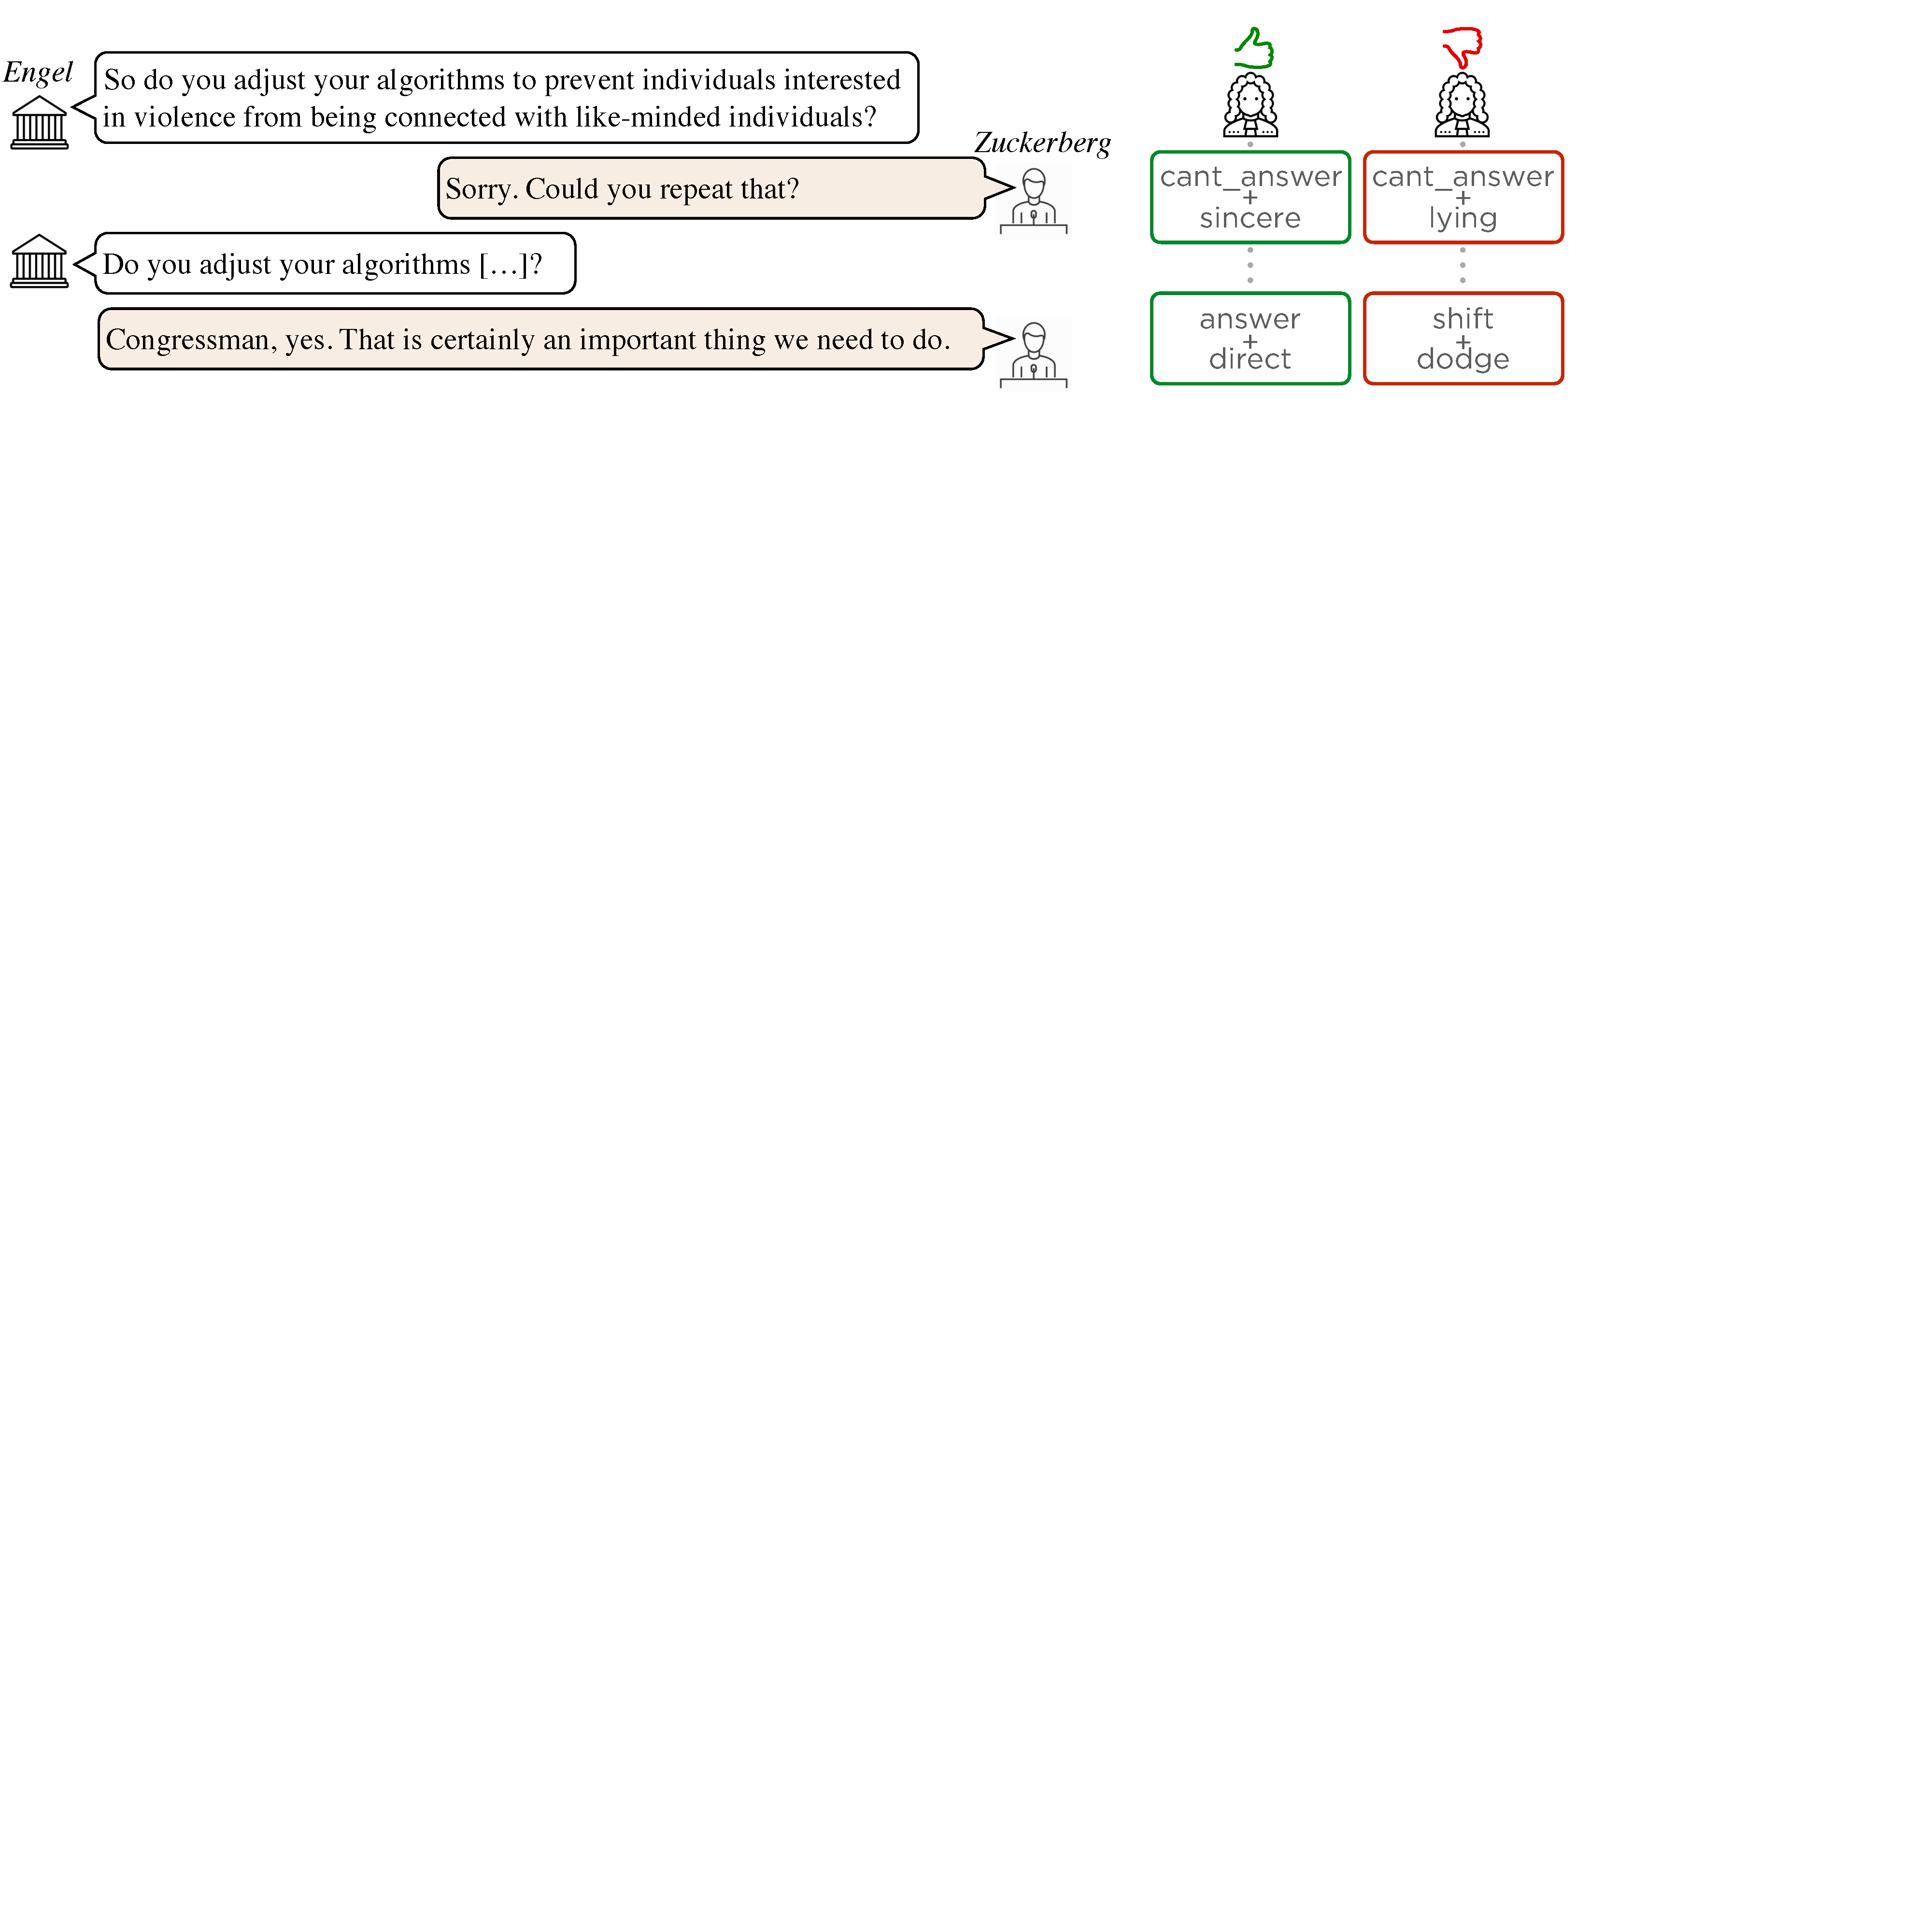
\includegraphics[scale=0.2]{plots/zuckerberg_conversation.pdf}
\vspace{-0.2em}
%[width=0.9\textwidth,height=50mm]
\caption{Conflicting interpretations of conversation acts+intents for witness responses in a U.S. congressional testimony.}
\label{fig:zuckerberg_conversation}
\vspace{-0.9em}
\end{figure}

In our example, the two annotators are the biased judges, and have differing judgments on what type of player Zuckerberg is (the first assumes \emph{sincere} and the second \emph{deceptive}). For Zuckerberg's first response, the conversation act is interpreted unambiguously: both annotators agree he is signaling he \texttt{can't answer} the question. The intent, however, is ambiguous, where the cynical annotator subjectively interprets the clarification question as \texttt{lying} in order to stall vs. being \texttt{sincere}. The second response yields both diverging conversation acts and intents: the first judge interprets the conversation act as an \texttt{answer} with the intent to provide a \texttt{direct} response, whereas the second judge perceives the conversation act as a \texttt{shift} to answer a different question with the intent to \texttt{dodge} the original, unfavorable question. Eliciting subjective interpretations of discourse moves allows us to create the first English discourse dataset with multiple, valid labels that are subjective and thus do not hold concurrently but vary depending on the annotator. We collect annotator sentiments towards the conversants as a rough proxy for the bias of the judge. We further elicit annotator explanations as a window into their rationalization process. A careful annotation protocol and qualification process ensures high quality annotators with a firm understanding of the task. Our dataset contains 6k judgments over 1k question-response pairs, and we find disagreements in roughly half of the data. Unlike our prior example, disagreements are not trivially attributable to differing sentiments. Uncooperative moves are sometimes warranted, but in other cases not tolerated, regardless of sentiment. The interpretation of the response is further influenced by its question. A qualitative analysis of annotator explanations helps pinpoint the utterance that annotators most attribute their judgments to, which can interestingly be the same across annotator sentiments but expressed with strikingly different uses of subjective language.

%understand sources of polarization and how group division manifests in language: Demszky 2019, Fryer 2017 (double belief updates for confirmation bias and polarization)

Understanding all the possible interpretations of a response could be useful in a practical setting of creating a more contextualized chat agent able to produce responses more personalized towards a particular user, but more generally aids in uncovering sociolinguistic aspects that are relevant to variations in discourse comprehension. With these future goals in mind, we propose the task of predicting the complete set of annotator labels for a given response. We find a transformer-based model outperforms other neural and linear models, and we confirm our assumption that incorporating the context (of both the conversation and the judge) helps the model make better predictions, as does accounting for the hierarchy in our label taxonomy (the conversation act/intent split). An error analysis reveals that context helps the model predict the smaller, more confusable classes. We also present preliminary results on predicting the level of disagreement for a response.

In summary, our contributions are the first English dataset with multiple yet valid subjective judgments of conversation acts and intents with rationales that showcase the linguistic creativity of subjective language; and the novel task of predicting all the possible interpretations of a conversational response where our model shows that taking into account the context of the question, the annotator and label hierarchy are helpful. The task together with the dataset present a valuable opportunity to understand perceptions of discourse in a non-cooperative environment.

\section{Background on speech act theory and Related work}
We first give an overview of speech act theory and its refinement, and then discuss related NLP tasks.

Our work focuses on capturing the judge's perception of the conversation act and its communicative intent. Conversation acts are a more general form of speech acts meant to account for phenomena specific to conversation that can encompass entire turns in a conversation \cite{Traum:1992}. Speech act theory can be traced back to \newcite{Austin:1962} describing performative actions, i.e., how we can do things with words. \newcite{Searle:1969} further refines performatives, but 
%into being composed of three parts: a locutionary force (what is said), an illocutionary force (what is done in the saying) and a perlocutionary effect (the consequence of the il/locutionary force). However,
their communication model fails to account for how the act is perceived by an observer (the judge in our framework). Subsequent work in speech act theory and planning extend this model to incorporate the cognitive context of an observer that includes the perceived \emph{communicative intent} underlying a speech act \cite{Cohen:1979,Pollack:1986}.

Because our data includes many forms of ostensible deception, we need to account for an insincere speaker, originally an ``abuse'' of the speech act theory. Nevertheless, even in non-cooperative settings, conversants adhere to the conventions of dialogue, or \emph{discourse obligations}, such as responding to a question \cite{Traum:1994,Potts:2008}. For this reason, we explicitly separate judgments on conversation acts (that usually fulfill a specific obligation) from communicative intents, which
%The intents traditionally communicate belief states, but in a game-theoretic view of (non-cooperative) conversation, a player more likely will not share their beliefs and instead have a goal to extract certain commitments from the other player \cite{Venant Asher 2015}. 
may be which can be perceived as insincere, and include forms of deception such as lying and dodging.  

Prior work has examined how writer intentions are often misaligned with reader perceptions \cite{Chang:2020}, which further motivates our focus on the reader (or judge). While our work focuses on subjectivity, ambiguity is studied across several NLP tasks with one recent work focusing on Natural Language Inference \cite{Pavlick:2019,Chen:2020}. The same is true in several discourse tasks \cite{Poesio:2019,Das:2017,Asher:2003,Versley:2011,Webber:2012,Webber:2019b}. One exception is \newcite{Scholman:2019} that investigates how resolving ambiguity in coherence relations can be attributable to different cognitive biases. However, our work focuses more generally on subjectivity instead of cognitive processes.   

% Dumitrache et al 2015 for semantic variation; Kairam and Heer 2016 for clustering workers; Palomaki et al 2018: argues for acceptable variation of annotations
%For the task of resolving anaphoric mentions, \newcite{Poesio:2019} estimates 10\% of the their crowdsourced coreference corpus is ambiguous, though they do not address the subjectivity of the differing interpretations. Psychology studies, however, do find people exhibit biases such as gender-stereotyping in coreference resolution as measured by longer reading times for pronouns when the antecedent (e.g., ``the surgeon'') is referred to with a mismatched gender-stereotypical pronoun (``her'') \cite{Cunnings:2014,Kennison:2003}.

%For the task of creating discourse trees in the RST framework, \newcite{Das:2017} finds ambiguities are most frequent in the step of labeling the tree, and more so for higher-level nodes that encompass larger spans of text.\footnote{The original RST framework distinguishes between subject matter and presentational relations, where multiple relations could apply to a single span \cite{Mann:1987}. However, this feature is orthogonal to allowing for multiple labels that are a result of \emph{subjective} judgments.} Even expert annotators labeling ostensibly less subjective texts (news articles) nevertheless have differing interpretations. The authors propose underspecified structures that leave the ambiguous part of the discourse unresolved (see also \newcite{Hanneforth:2003}). However, this approach abstracts away the different interpretations that we are specifically interested in modeling.

%In the lexicalized approach of PDTB, discourse connectives are often ambiguous as to what discourse relation they signal (other forms of ambiguity are discussed in \newcite{Webber:2019b}). While PDTB allows for multiple relations, these are meant to be concurrent vs. \emph{alternative} senses (i.e., a single annotator would interpret both senses). \newcite{Webber:2012} argues that disagreements in PDTB stem from issues in the annotation scheme (a revised scheme in PTDB 3.0 corrects some of these ambiguities \cite{Webber:2019b}). However, other work does find a subjective bias in these kinds of disagreements.

NLP tasks related to our work include dialog act classification, intent detection, deception detection and argumentation, though we importantly note these predict only a single interpretation. Dialog acts are closely related to conversation acts that apply at the utterance level. Classification models typically employ a hierarchical structure to focus on word, utterance, and conversation level representations, and frame the task as a sequence labeling problem to incorporate dependencies between utterances \cite{Chen:2018}. In our work, we employ a hierarchical model to account for the levels in our label taxonomy, and leave sequential modeling for future work. Intent detection is traditionally applied to human-computer scenarios for achieving a specific task such as booking a flight. 
%An utterance is assigned to one or more pre-defined intents (note that multiple labels are meant to hold concurrently not alternatively). 
%Separately, the agent must fill semantic slots such as the booking time to correctly parse the human's utterance. Slot-filling and intent prediction are strongly correlated and modeling them jointly is mutually beneficial \cite{Li:2018}.
%Similar to dialog acts, models also exploit the sequential dependence of intents \cite{Gangadharaiah:2019}. 
Our conversation data is not task-oriented, and we thus define our intents more closely aligned with the beliefs in the sincerity of the speaker. Deception is the intent to create a belief in the listener that the speaker knows is false \cite{Girlea:2017}. Detection of deception is, unlike many other NLP tasks, challenging even for humans \cite{Ott:2011}.
%In the absence of context such as motive and situational familiarity, participants in psychology experiments perform only slightly better than chance \cite{Levine:2019} . 
Most datasets consist of instructed lies, where participants are told to lie. 
%Models derive  linguistic features such as the use of hedge words or greater specificity . 
Our work contains naturally-occurring deception and we adopt a broader view of deception beyond lying to include more covert mechanisms such as being deliberately vague or evasive \cite{Clementson:2018}, which are frequent in political discourse \cite{Bull:2008}. Finally, our framing of conversations as a game in a non-cooperative setting is more closely aligned with argumentation, where conversants have opposing goals. Argumentation mining typically requires highly-trained annotators to identify argument components such as claims and premises, but recent work aims to decompose the task into intuitive questions for crowdsourcing \cite{Miller:2019}, which we use as inspiration for our annotation schemes that assume little to no training. However, unlike our work, their task is not framed as being subjective. Closer to our work, other studies focus on argument persuasiveness, or whether an audience switches sides after watching an argument \cite{Zhang:2016,Durmus:2018}. \newcite{Durmus:2018} finds prior beliefs of the audience play a strong role in their ability to be persuaded, which further motivates our focus on the annotator's bias.
 
\section{Dataset: Subjective acts and intents in conversational discourse}
We create the first dataset in English with multiple, subjective interpretations of discourse. Recalling our example in Figure \ref{fig:zuckerberg_conversation}, we focus on responses to questions and how these responses are perceived to address the question (the \emph{conversation act}, such as Zuckerberg saying he \texttt{cant\_answer}) and the intent behind choosing that form of response (the \emph{communicative intent}, such as one annotator believing the intent was \texttt{sincere}). As our source of data, we choose the question-answer portions of U.S. congressional hearings for several reasons: they contain political and societal controversy identifiable by na{\"i}ve crowdsourced workers, they have a strong signal of ambiguity as to the form and intent of the response, and the data is plentiful.\footnote{Transcripts do not include intonation or gestures and thus a certain amount of information is lost from the original discourse.} See Appendix \ref{sec:app_subjective} for a detailed dataset statement.

\begin{table}
\centering
\small
\vspace{-1em}
\begin{tabular}{c p{1.5cm} p{1.5cm} p{1.5cm} p{1.5cm} p{1.5cm}}
\toprule
item  & \#sents/turn     & \#tokens/turn &total sents &total toks&total spkrs     \\ 
\midrule
question  &4.1  &81.5 &4096 &82582 &91  \\
response &2.6 &47.0 &2634 &48831 &20 \\
\bottomrule
\end{tabular}
\vspace{-0.5em}
\caption{Dataset statistics.}
\label{tab:subj_corpus_stats}
\end{table}

\subsection{Dataset creation}
Congressional hearings are held by congressional committees in order to gather information about specific topics or issues before legislating policies. Hearings usually include testimonies and interviews of witnesses. We focus on hearings that interview a single witness and that exceed a certain length ($>$100 turns) as a signal of argumentative discourse. To ensure a variety of topics and political leanings are included, we sample a roughly equal number of hearings from 4 Congresses (113th-116th) that span the years 2013-2019. For each hearing, we extract the interview portion, identify turns in conversation and which turns have a question. We then split the data into question-response pairs and extract the first 50 pairs from each hearing. Each data point consists of a question (from a politician) followed by a response (from the witness). The dataset statistics are summarized in Table \ref{tab:subj_corpus_stats}.

\subsection{Dataset annotation} 
\label{sec:subj_annotations}
We collect labels through the Amazon Mechanical Turk crowdsourcing platform. The task consists of three exercises: judging the question, judging the response, and reporting annotator sentiment (see Appendix \ref{sec:app_anno} for screenshots and additional details). Each HIT consists of five question-response pairs in sequential order from the same hearing (we group them to preserve continuity of the conversation while not overloading the annotator). To ensure a variety of annotator viewpoints with different biases, we collect 7 judgments for each HIT.\footnote{During the pilot study, we experimented with increasing the number of judgments (up to 11 annotators) but found the number of chosen labels remains stable. We thus scaled back to 7 for the full data collection.} We recognize that crowd-sourced workers and thus our collected judgments are not representative of the U.S. population \cite{Difallah:2018}. 

\subsubsection{Annotations}
For each question-response pair we collect three pieces of information: the question label (not used in this work), the response label, and an explanation. At the end of each HIT, we collect two pieces of information: the annotator's sentiment towards the questioners, and the annotator's sentiment towards the witness.\footnote{We collect sentiments at the \emph{end} of the HIT because we do not expect annotators to have a priori an understanding of the issue being discussed in the hearing or a high level of familiarity with the questioners or the witness.}

\begin{table}[]
\small
    \centering
    \begin{tabular} {p{0.1cm} >{\raggedright\arraybackslash}p{6.0cm} >{\raggedright\arraybackslash}p{3.4cm}}
    \toprule
(1) &\textbf{Q: } How much of the financing was the Export-Import Bank responsible for? & \textbf{R: }We financed about \$3 billion.\\\midrule
(2) &\textbf{Q: } If you were properly backing up all the information \textit{\uline{required under the Federal Records Act, which would include the information she selected to have and apparently deleted from the exchange server}}, you would have had all of those emails in your backup, \textit{\textbf{wouldn't you}}? & \textbf{R: } All emails are not official records under any official records act.\\
\midrule
(3) &\textbf{Q: }So you're not willing to say that it doesn't meet due process requirements at this point? & \textbf{R: } 
Well, what I'd like to do is look at the procedures that are in place before I made a constitutional determination about due process.\\
\bottomrule
    \end{tabular}
    \vspace{-.5em}
    \caption{Different forms of questions lead to different kinds of responses: (1) an objective, information-seeking question with a direct answer. (2) A loaded question with a \uline{\textit{presupposition}} and a \textbf{\textit{leading tag question}}, where the responder fails to provide a direct yes/no answer because they reject the presupposition. (3) A declarative question where the questioner commits to an unfavorable view of the responder, and the response is an indirect answer.}
    \label{tab:subj_questions}
\end{table}

\paragraph{Question}
We ask the annotator to label the question, as it can influence the form and perception of the response. For example, an objective information-seeking question lends itself to a direct answer (example (1) of Table \ref{tab:subj_questions}). On the other hand, a \emph{loaded} question contains presuppositions or assumptions \cite{Walton:2003}, but canceling these presuppositions means the response will not have a semantic answer, resulting in an indirect answer \cite{Groenendijk:1984} as in example (2) of Table \ref{tab:subj_questions}. \emph{Leading} questions, often in the form of declarative questions, are conducive to a particular answer \cite{Bolinger:1957}. These types of questions imply the questioner is committed to the question's proposition, and a pragmatic listener (or judge) will assume the questioner has a reliable source for this commitment, helping the listener interpret the questioner's intent \cite{Gunlogson:2008} (though this rule may fall apart in non-cooperative settings). Leading questions also lead to indirect answers if the responder has to challenge these commitments, as in example (3) of Table \ref{tab:subj_questions}.

For judging the question, we ask the annotator to make a binary (yes/no) decision on whether the politician includes a leading question, controversial assumption or attack (our task does not use the term ``presupposition'' to avoid linguistic jargon). If the annotator chooses yes, we assign a label of \texttt{attack}. If the annotator chooses no, they are presented with a second binary decision to judge whether the politician is favoring the witness. If the annotator chooses yes, the label is \texttt{favor}. If the annotator chooses no for both questions, we infer the label of the question to be \texttt{neutral}. 

\begin{figure}[t]
\centering
\vspace{-1.0em}
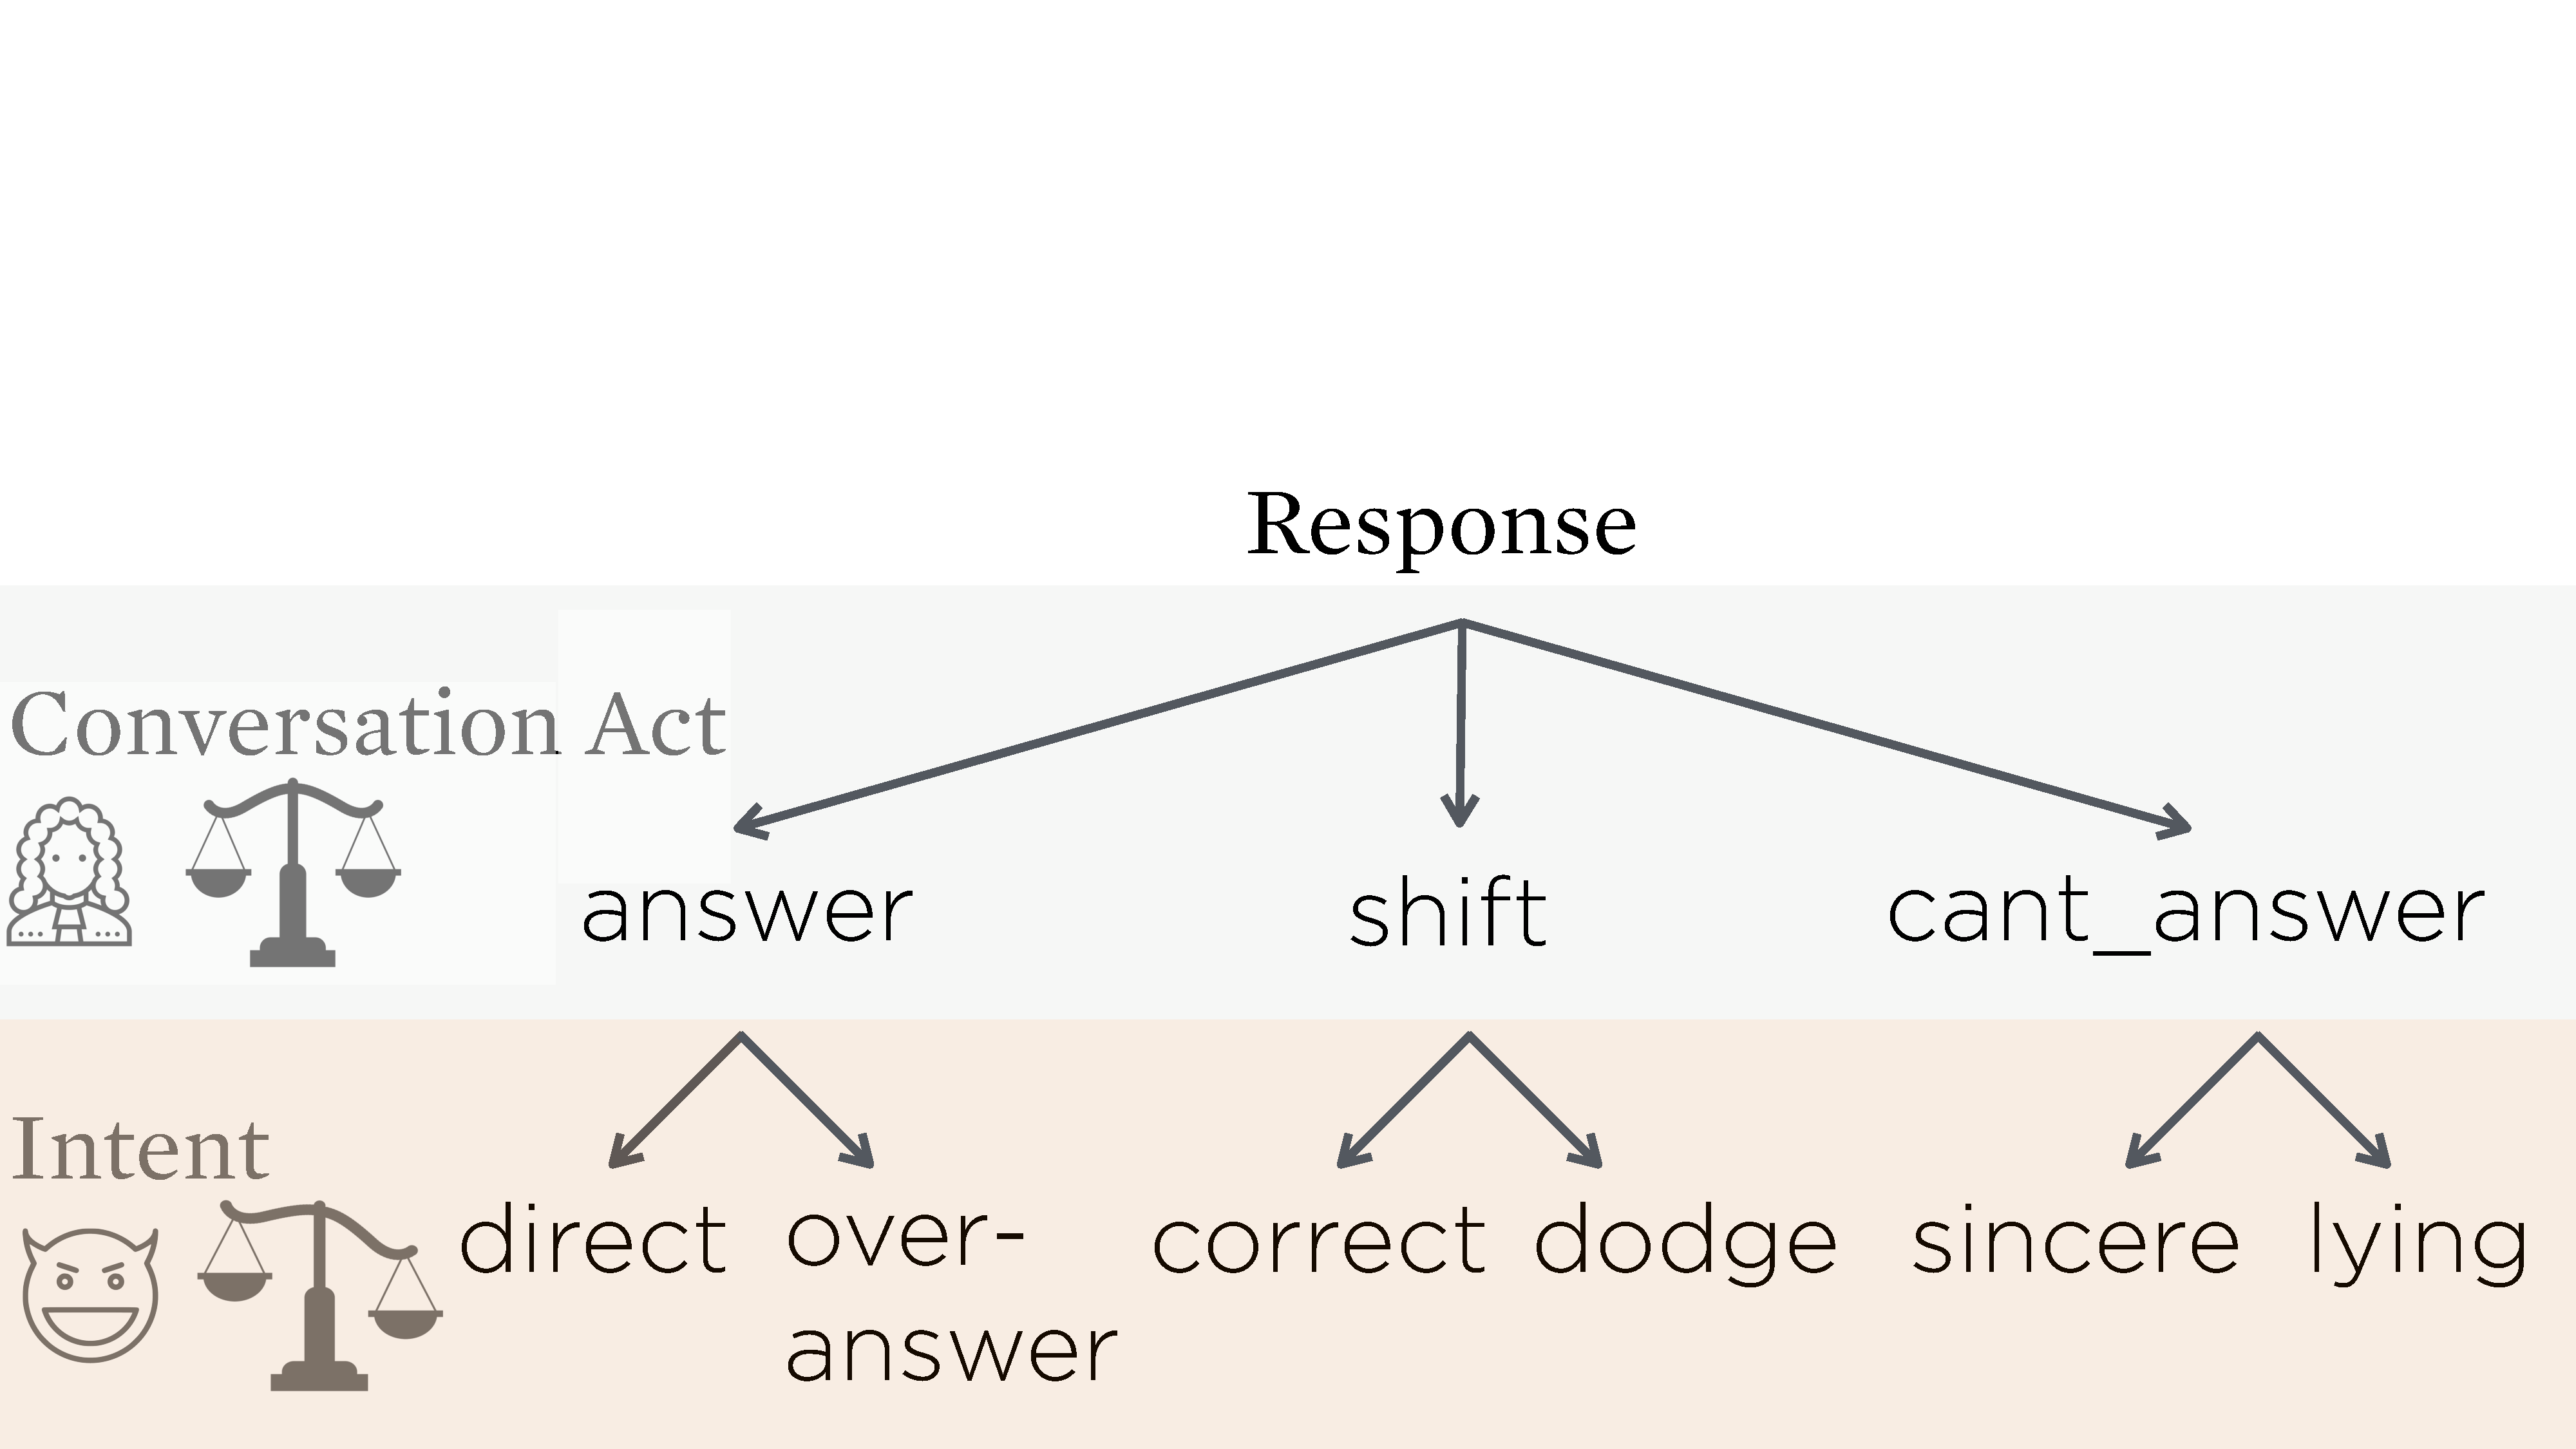
\includegraphics[scale=0.12]{plots/response_taxonomy.pdf}
\vspace{-0.5em}
\caption{Hierarchical taxonomy of the perceived conversation act and intent for a response.}
\label{fig:response_taxonomy}
\end{figure}

\paragraph{Response} For judging the response, we combine conversation acts with communicative intents as in Figure \ref{fig:response_taxonomy} (in the spirit of the compositional semantic framework of \newcite{Govindarajan:2019}). In accordance with the discourse obligations of a conversation, a witness must respond in some form to a question \cite{Traum:1994}. The function of the response is captured by the perceived \emph{conversation act}, and is meant to be a more objective judgment (e.g., recognizing that Zuckerberg is using the \emph{`can't answer'} form of a response, regardless of whether you believe him). This conversation act constitutes the top layer of the taxonomy. The bottom layer is the perceived \emph{intent} underlying that conversation act, and is meant to be subjective. The conversation acts include the standard \texttt{answer} and \texttt{cant\_answer}. Inspired by work on answerhood \cite{Ginzburg:2019,DeMarneffe:2009,Groenendijk:1984} and evasion in political discourse \cite{Gabrielsen:2017}, we also include a more nuanced view of answering the question where giving a partial answer or answering a different question is labeled as \texttt{shift}. The intents hinge on whether the annotator believes the witness's conversation act is sincere or not. For \texttt{answer}, the annotator may believe the intent is to give a \texttt{direct} answer, or instead an \texttt{overanswer} with the intent to sway the reader.\footnote{Overanswering with the intent to be helpful was included in our original taxonomy but then eliminated because of sparsity.} If \texttt{shift}ing the question, the reader may believe the responder is \texttt{correct}ing the question (e.g., to reject a false presupposition) or is attempting to \texttt{dodge} the question. If the witness says they \texttt{cant\_answer}, the reader may believe the witness is \texttt{sincere} or is \texttt{lying}.

The annotation task implements a series of nested questions that mimic the hierarchy of the label taxonomy, which we then map to conversation act and intent labels (Figure \ref{fig:subj_amt_screenshots_nested} in Appendix \ref{sec:app_anno}).
%\footnote{An initial pilot of the task that required annotators to learn the label taxonomy proved onerous and confusing.} 
That is, we first ask how the witness responds to the question (conversation act) and then what is the intent and combine these into a single response label.

\paragraph{Explanation} We ask annotators for an \emph{explanation} of their choices in order to elicit higher quality labels \cite{McDonnell:2016} and for use in the qualifying task as explained later. 

\paragraph{Sentiment} At the end of the HIT, we ask the annotator to rate their sentiment towards the politicians and towards the witness on a 7-point scale (we later collapse these into 3 levels: negative, neutral, positive). These ratings can provide a rough proxy for annotator bias. 

\subsubsection{Worker qualification}
Because the task requires significant time and cognitive effort, we establish a qualification process to filter out spammers or annotators who do not understand the task (in addition to the standard requirements: $>$95\% approval rating, $>$500 approved HITs, and living in the US for greater familiarity with the political issues). For the qualifying task, we present question-response pairs that were explained as examples in the instructions as well as unambiguous cases as far as the conversation act (e.g., a response of `Yes' can only be construed as an answer). We also examine the explanations and response time of the annotator (see Appendix \ref{sec:app_anno} for complete criteria). 

This rigorous process yielded high quality data from 68 annotators who were genuinely engaged with the task. Qualified workers were compensated an average of \$1.20 per HIT. On average, an annotator labeled 91 question-response pairs, with 4 superannotators who provided labels for half of the data. During post-processing, we discard single-vote annotations (where only one annotator voted for a label on the same response). The annotated dataset consists of 1000 question-response pairs with 6,205 annotations (3-7 annotations per item) on the first 50 question-responses from each of 20 congressional hearings. 

\begin{figure}
\centering
\includegraphics[scale=.47]{plots/subj_response_dist.pdf}
\vspace{-1.0em}
\caption{Distribution of annotation labels for responses.}
\label{fig:subj_response_dist}
\end{figure}

% \begin{figure}
% \RawFloats
% \centering
% \begin{minipage}{.5\textwidth}
%   \centering
%   \includegraphics[scale=.4]{plots/subj_response_dist.pdf}
%   \vspace{-1.0em}
%   \captionof{figure}{Distribution of annotation labels for responses.}
%   \label{fig:subj_response_dist}
% \end{minipage}%
% \hspace*{1.4em}
% \begin{minipage}{.5\textwidth}
%   \centering
%   %\vspace{1.3em}
%   \includegraphics[scale=.4]{plots/subj_witness_sentiment_dist.pdf}
%   \vspace{-1.0em}
%   \captionof{figure}{Distribution of (coarse-grained) annotator sentiment towards the witness.}
%   \label{fig:subj_witness_sentiment_dist}
% \end{minipage}
% \end{figure}

\subsection{Annotated Dataset Characterization}
In this section, we explore the annotated dataset to both confirm the validity of the data and to gain a deeper understanding of it. We mainly focus on the annotations for the witness response (Figure \ref{fig:subj_response_dist}) and sentiment towards the witness.
%(Figure \ref{fig:subj_witness_sentiment_dist}, skewing slightly negative).

We first confirm our assumption that disagreements do exist, and then show these are in fact genuine and not noise. We then explore patterns in the annotator sentiments towards the witness and how these are related to the labels they chose. 

% \begin{wrapfigure}{ri}{0.3\textwidth}
% \centering
% \vspace{-2.2em}
% \includegraphics[scale=.48]{plots/subj_witness_sentiment_dist.pdf}
% \vspace{-1.em}
% \caption{Distribution of annotator (coarse-grained) sentiment towards the witness.}
% \label{fig:subj_witness_sentiment_dist}
% \end{wrapfigure}

\begin{figure}
 \centering
 \vspace{-1.2em}
  \begin{subfigure}{.3\textwidth}
  \centering
  \includegraphics[scale=0.28]{plots/subj_disagreement.pdf}
  \vspace{-.3em}
  \caption{all hearings}
\end{subfigure}%
  \begin{subfigure}{.3\textwidth}
  \centering
  \includegraphics[scale=0.3]{plots/subj_disagreement_kerner.pdf}
  \vspace{-.3em}
  \caption{Violations of the Hatch Act}
\end{subfigure}%
\begin{subfigure}{.3\textwidth}
  \centering
  \includegraphics[scale=0.3]{plots/subj_disagreement_whitaker.pdf}
  \vspace{-.3em}
  \caption{Oversight of the Dept. of Justice}
\end{subfigure}
\vspace{-0.5em}
  \caption{Disagreements over the entire dataset (a) compared with two hearings having markedly more (a) or less (b) disagreement.}
  \label{fig:subj_disagreement_hearing}
  \vspace{-.3em}
\end{figure}

\paragraph{Is there disagreement?} An initial concern with modeling multiple interpretations was whether crowdsourced workers would actually have sufficiently different viewpoints. A demographic study in \newcite{Difallah:2018} found turkers were younger and lower income earners than the average U.S. population, factors which are also correlated with certain political leanings. However, we do find there is sufficient disagreement, in part because disagreements often stem from more nuanced viewpoints that don't fall along party lines.
%\footnote{The pilot task asked the annotator for an opposing viewpoint label in addition to their own, but this was later removed after finding it was unnecessary (and likely problematic to ask people to adopt other mindsets).} 
Figure \ref{fig:subj_disagreement_hearing} (a) shows people disagree on roughly half the data, although this trend can vary considerably from one hearing to the next as shown in (b) and (c).

\begin{figure}
\vspace{-1.2em}
\centering
\includegraphics[scale=0.4]{plots/subj_kripp_bar.pdf}
\vspace{-.3em}
  \caption{IAA on the \textit{disagreement} subset for all annotators (left) increases when grouped by sentiment (right). The dashed orange line is the IAA for the entire dataset.}
  \label{fig:subj_kripp}
\end{figure}

\paragraph{Is disagreement real or noise?} In spite of our rigorous qualification process, it is still possible qualified workers construed the labels differently. In order to understand whether the disagreements are genuine or due to noise, we compare the inter-annotator agreement (IAA) of different annotator groups and examine what labels the workers disagree on the most. 

IAA measured with Krippendorff's $\alpha$ over the entire dataset is 0.494, considered `moderate' \cite{Artstein:2008}, but also reasonable considering we expect and elicit disagreement. Importantly, we find higher agreement on the conversation act (0.652) compared to the intent (0.376 in binarized form), confirming our intuition that the top-level label is more objective than the bottom-level one. One might expect annotators with similar sentiments towards the witness to agree more with each other than with others, and particularly so for the responses with disagreements. We partly confirm this intuition on the disagreement data in Figure \ref{fig:subj_kripp}: grouping annotators by their sentiment increases agreement, but not much. In fact, sentiment is a more complicated signal that we explore further in the next section.  

\begin{table}
\centering
\small
\begin{tabular}{>{\raggedright\arraybackslash}ll}
\toprule
Disagreement  &Percent\\ 
\midrule
\texttt{answer+{\color{blue}direct}} vs. \texttt{shift+{\color{red}dodge}} &29.8\\
\texttt{shift+{\color{blue}correct}} vs. \texttt{shift+{\color{red}dodge}} &15.4 \\
\texttt{answer+{\color{blue}direct}} vs. \texttt{answer+{\color{red}overans}} &10.5 \\
\texttt{cant\_ans+{\color{blue}sincere}} vs. \texttt{cant\_ans+{\color{red}lying}} &\phantom{0}9.0 \\
\texttt{answer+{\color{blue}direct}} vs. \texttt{shift+{\color{blue}correct}} &\phantom{0}7.3 \\
\texttt{answer+{\color{blue}direct}} vs. \texttt{shift+{\color{blue}correct}} vs. \texttt{shift+{\color{red}dodge}}&\phantom{0}6.7\\
\bottomrule
\end{tabular}
\vspace{-.3em}
\caption{Most frequent disagreements in the dataset and their percent; sincere intents in {\color{blue}blue} and insincere in {\color{red}red}.}
\label{tab:subj_label_set_disagree}
\end{table}

% \begin{wrapfigure}{ri}{0.37\textwidth}
% \centering
% \includegraphics[scale=0.4]{plots/subj_label_set_disagree.pdf}
%   \caption{Most frequent response label disagreements calculated as a percent of all disagreements.}
%   \label{fig:subj_label_set_disagree}
% \end{wrapfigure}

% \begin{table}[t]
% \centering
% \small
% \begin{tabular}{p{3.32cm}p{3.9cm}|l >{\raggedright\arraybackslash}p{4.7cm}}
% \toprule
% Question  & Response     &Label &Explanation  \\ 
% \midrule
% \multirow{4}{=}{Why is FaceBook censoring conservative bloggers? Facebook called them unsafe. What is your response to that?} & \multirow{4}{=}{Congressman, in that specific case, our team made an enforcement error, and we have already gotten in touch with them to reverse it.} & \texttt{answer+direct} & witness acknowledges and \uline{answers the question honestly} \\
% &&&\\
% && \texttt{shift+dodge} & He answered about 2 individual cases, but \uline{did not address the overall issue of partisan censorship}\\
% \bottomrule
% \end{tabular}
% \vspace{-.7em}
% \caption{Example of the most frequent disagreement (answer+direct vs. shift+dodge), where the underlined portions of the explanation highlight the differing interpretation of intent.}
% \label{tab:subj_disagree_example}
% \end{table}

We next explore the labels that annotators most frequently disagree on. Table \ref{tab:subj_label_set_disagree} shows annotators mostly disagree on one of two labels with opposing intents, though often the conversation act is the same (e.g., \texttt{shift+correct} vs. \texttt{shift+dodge}). This result is encouraging, showing annotators have a shared understanding of the label definitions and further motivating our label taxonomy (Figure \ref{fig:response_taxonomy}). Explanations reflect disagreements as we later show in our qualitative analysis. Finally, contradictory disagreements such as \texttt{answer} vs. \texttt{cant\_answer}, where a witness would be judged to provide an answer while also saying they can't answer, are rare ($<5$\% of all disagreements).


\begin{table}[t]
\centering
\small
    \begin{tabular}{>{\raggedright\arraybackslash}p{5cm} >{\raggedright\arraybackslash}p{2.5cm} p{1.5cm} p{1cm}}
    \toprule
Question &Response &Unanimous Label &Sentm. Dist.\\
\midrule
Let's talk about your small business jobs for a second. We used to be on the Small Business Committee, and we had a couple of different definitions for what was a small business. What was yours? & What was my--say that again, sir? &\texttt{cant\_answer+} \texttt{sincere} &\raisebox{-\totalheight}{\includegraphics[scale=.2]{plots/subj_unambig_example.pdf}}\\
And you spoke to their CEO immediately? &We shut down the app. We demanded-- & \texttt{shift+ dodge} &\parbox[c]{1em}{\includegraphics[scale=.2]{plots/subj_unambig_example.pdf}}\\
    \bottomrule
    \end{tabular}
    \vspace{-.4em}
    \caption{Example of `winning sincerity' (top) and `losing evasiveness' (bottom) where all annotators agree on the same label, even when it conflicts with their sentiment towards the witness.}
    \label{tab:subj_unambig_example}
\end{table}

\paragraph{Is sentiment predictive of intent?} We have pointed out how the annotator's sentiment towards the witness can help explain the label they choose. Is the sentiment then an easy predictor of intent or is it a more complicated signal? A correlation study shows they are in fact only weakly correlated (correlation ratio $\eta$=0.33 for coarse-grained sentiment).
%\footnote{The correlation ratio $\eta$ is equivalent to Pearson’s correlation coefficient except that it can be applied to categorical data. The $\eta$ ranges from 0 to 1}. 
There are two reasons for this result: responses  often have an unambiguous interpretation regardless of annotator sentiment, and annotator sentiment towards the witness typically fluctuates throughout the hearing.


For unambiguous responses, the most common label (58\%) is \texttt{answer+direct}, where direct answers leave little room for interpretation (e.g., `Yes, that is correct.'). More interestingly, a smaller portion of unambiguous items (10\%) involve annotators interpreting intents that conflict with their sentiment towards the witness. Recalling the conversation-as-a-game theory \cite{Asher:2003}, we term these cases as either `winning sincerity' (where skeptical annotators agree the witness is sincere) or `losing evasiveness' (where favorable annotators agree the witness is evasive), listing two representative examples in Table \ref{tab:subj_unambig_example}. In the `winning sincerity' example, the witness asks for clarification, and even the negatively-biased annotators interpret the response as sincere (in contrast with Zuckerberg's clarification request that was interpreted as lying). These `winning sincerity' clarification requests have word overlaps with the question, and may thus be perceived as less vague. In the `losing evasiveness' example, the witness shifts the question, and even positively-biased annotators interpret the intent as evasive (not correcting). In many of these cases, the witness is cut off by the questioner (transcribed as `--'). We speculate the positively-biased annotator is influenced by the negative judgment of the questioner. While these are small phenomena, they illustrate the nuances of signaling sincerity and how they interact with the annotator's sentiment towards the witness.

% \begin{wrapfigure}{ri}{0.37\textwidth}
% \centering
% \includegraphics[scale=.4]{plots/subj_sentiment_flips.pdf}
% \caption{Annotators flip their sentiment towards the witness up to four times in this hearing. Each annotator is depicted as a different color (not all annotators annotate every HIT).}
%   \label{fig:subj_sentiment_flips}
% \end{wrapfigure}

For the annotator's sentiment across a hearing, a simplifying assumption is that it remains constant (recall the sentiment is reported at the end of each HIT, and HITs are presented to annotators in almost the same order as the original hearing). In practice it does not (59\% of annotators that label more than one HIT change their sentiment). 
%As a more extreme case of wavering sentiment, we focus on cases where the sentiment flips, that is, changes from positive to negative or vice versa (ignoring changes to neutral). We find sentiment flips are still common (38\% of annotators) and happen in every hearing, even up to 4 times in one particular hearing. 
As one annotator explained,``When he [the witness] said that, I got a different attitude towards him.'' 
%We also note different annotators have higher or lower propensity to change sentiments, regardless of the number of HITs they annotate.\footnote{While my work does not focus on understanding the source for these differences, prior work shows the propensity of people to change their beliefs can be traced back to personality traits \cite{Lukin:2017}.} 

Our characterization of the dataset shows there is a considerable amount of genuine disagreement, usually with opposing intents. Interestingly, these disagreements are only partly attributable to differences in annotator sentiment. We find cases where annotators with a negative sentiment nevertheless perceive a sincere intent (and vice versa). Furthermore, sentiment often fluctuates across a hearing, and can be influenced by what is said during the hearing.

\subsection{Qualitative Analysis of Explanations}
The explanations are a rich source of data for understanding annotator interpretations, with evidence they are applying their personal beliefs (`Bankers are generally evil') and personal experiences (`I have watched hearings in congress'). We conduct a qualitative analysis to gain insight into the differing interpretations.  The explanations are free-form, but annotators sometimes quote parts of the response (and question). Interestingly, multiple annotators sometimes quote the same text, yet arrive at completely opposite labels, as in the examples in Figure \ref{fig:subj_explanations}. Studying these cases offers a window into what part of a discourse may trigger a subjective view in observers, and how they express their view. 

\begin{figure}
    \centering
    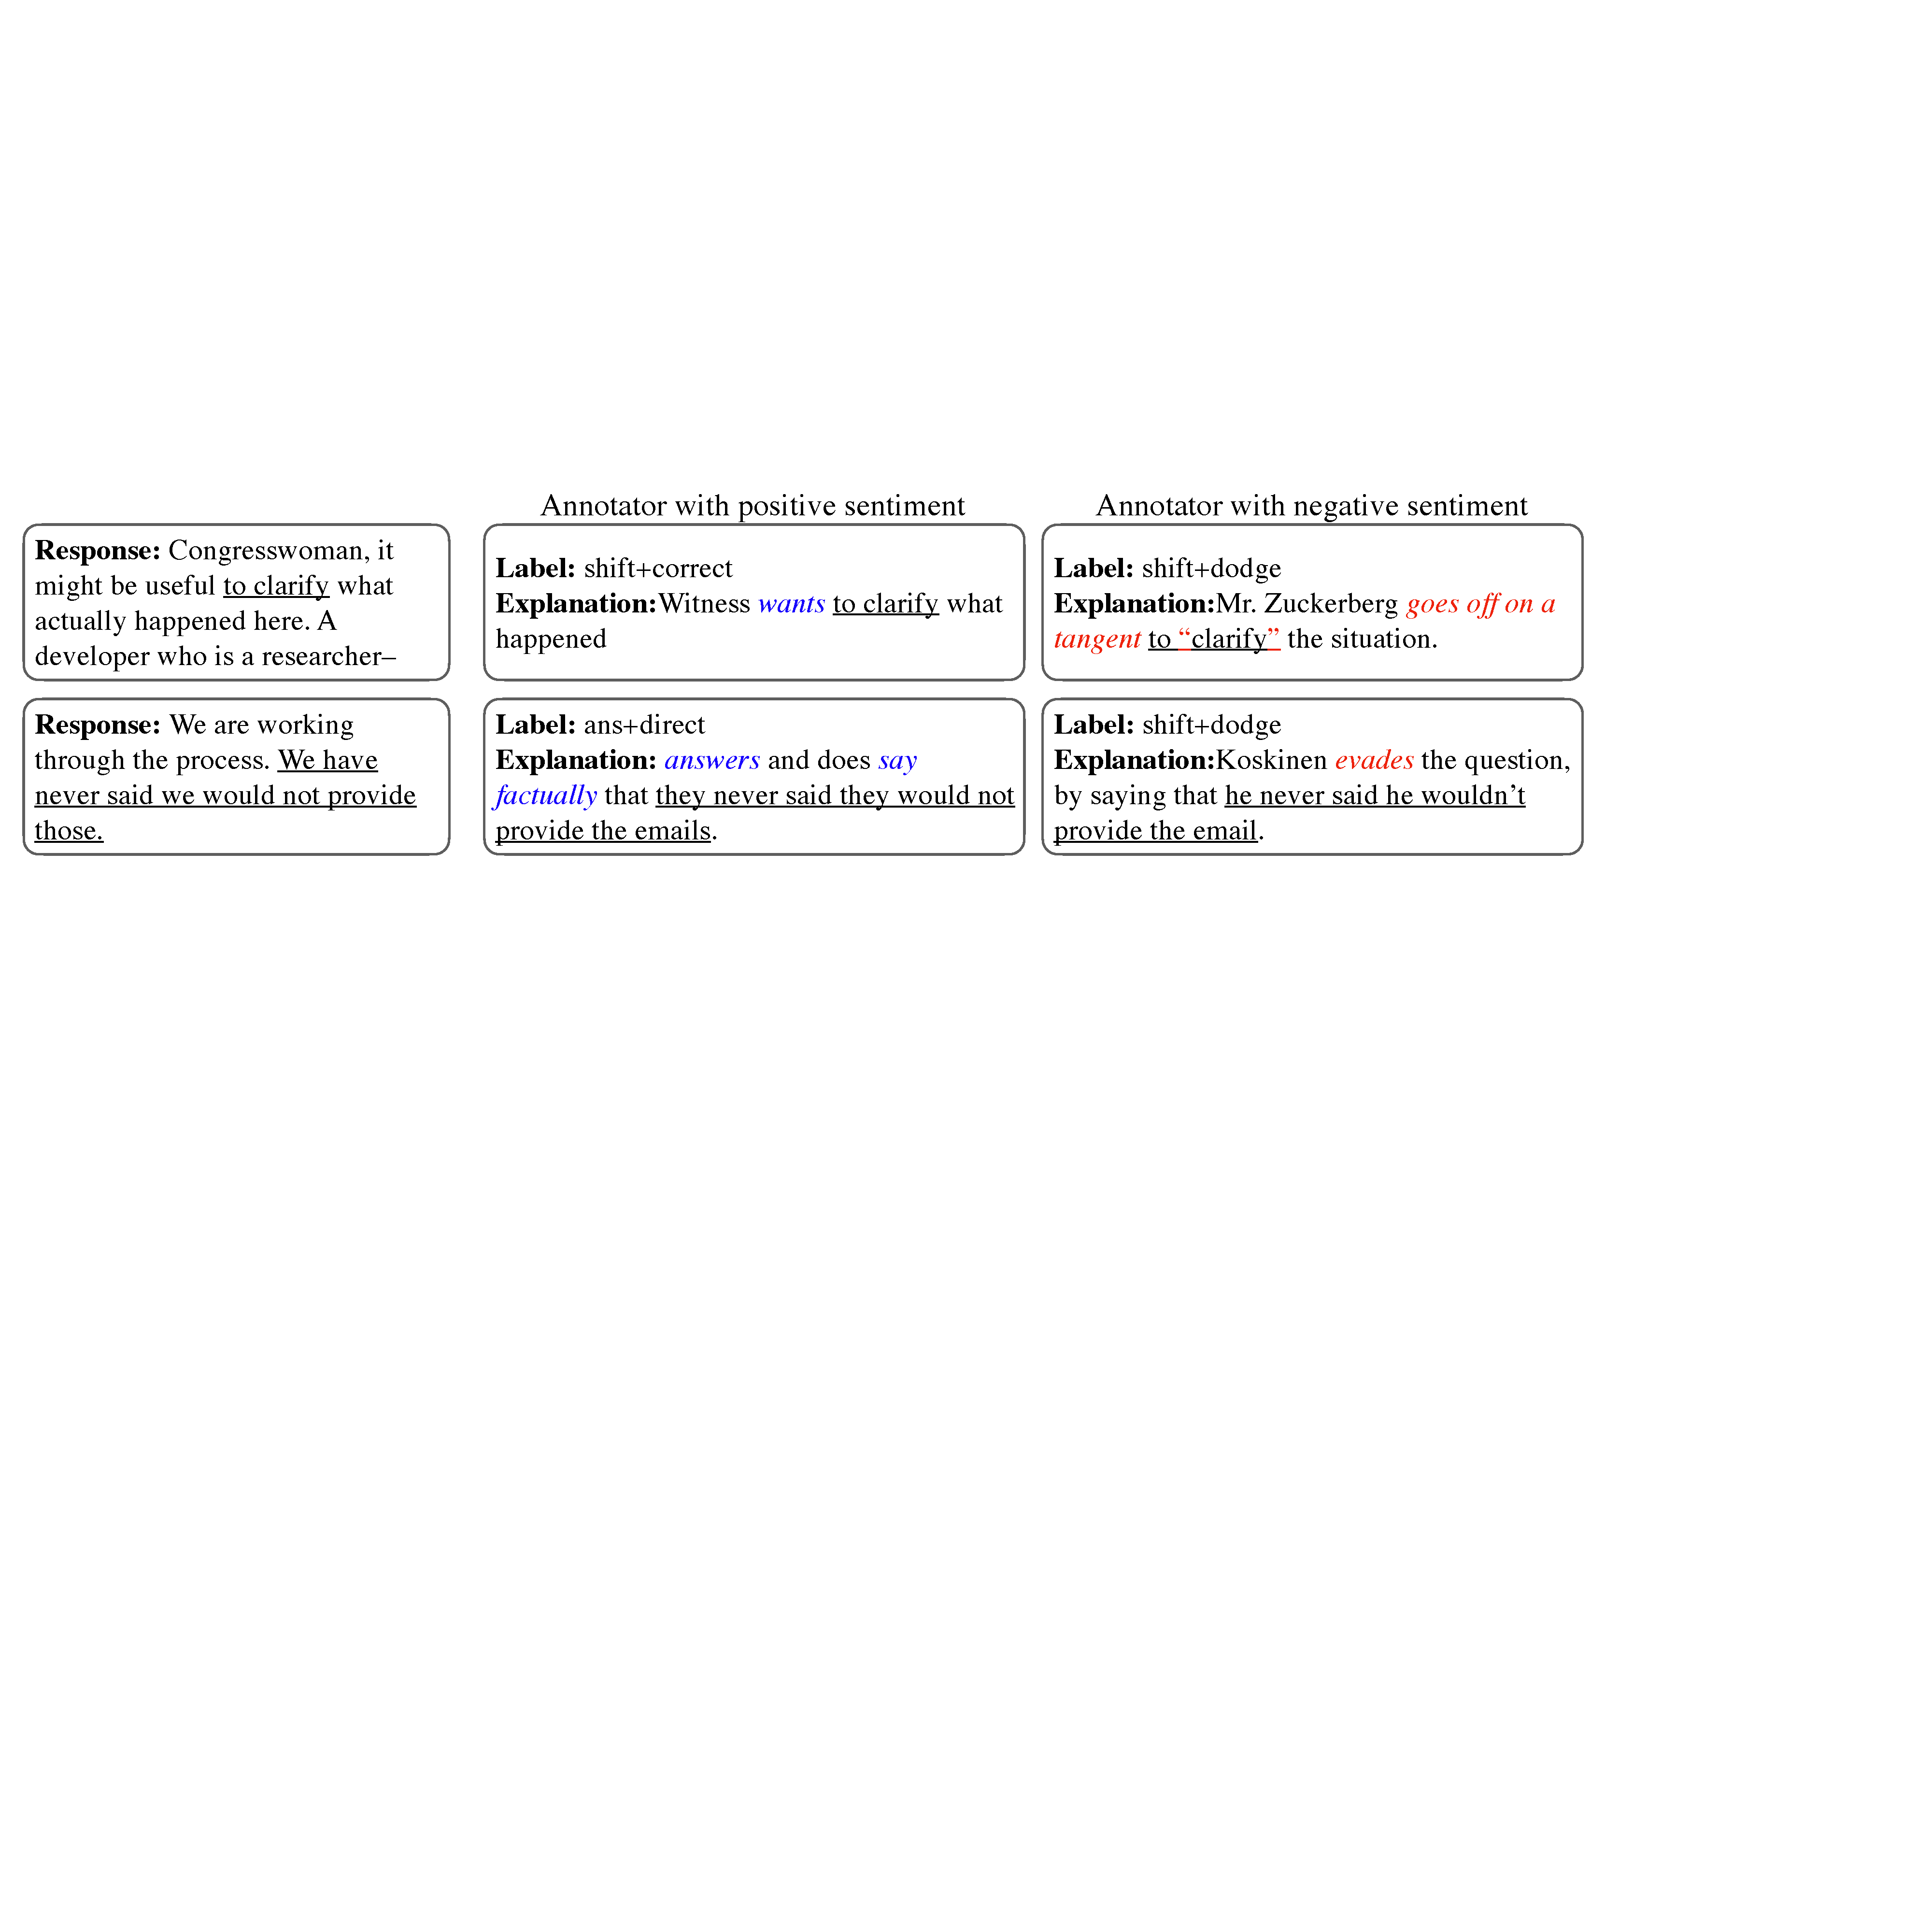
\includegraphics[scale=0.21]{plots/explanation_quotes.pdf}
    \vspace{-2.0em}
    \caption{Explanations from annotators with opposing interpretations quoting the same  response text (\uline{underlined}) with subjective language in {\color{blue}blue} (neutral, positive) and {\color{red}red} (negative).}
    \label{fig:subj_explanations}
\end{figure}

% \begin{table}[]
% \centering
% \small
% \begin{tabular}{@{}p{0.1cm} >{\raggedright\arraybackslash}p{3.8cm} p{0.9cm} >{\raggedright\arraybackslash}p{4cm} p{0.9cm} >{\raggedright\arraybackslash}p{4cm}@{}}
% \toprule
% \multirow{2}{*}{} & \multirow{2}{*}{Response} & \multicolumn{2}{c}{Sincere witness} & \multicolumn{2}{c}{Deceptive witness} \\ \cmidrule(lr){3-4} \cmidrule(lr){5-6} 
%  &  & \multicolumn{1}{c}{Label} & Explanation & Label & Explanation \\ \midrule
% \multicolumn{1}{c}{(1)} &
% Congresswoman, it might be useful \uline{to clarify} what actually happened here. A developer who is a researcher-- & shift+ correct &Witness {\color{blue}\emph{wants}} \uline{to clarify} what happened[\dots]  &shift+ dodge  &Mr. Zuckerberg [\dots] {\color{red}\emph{goes off on a tangent}} \uline{to {\color{red}\emph{``}}clarify{\color{red}\emph{''}}} the situation.\\
% \multicolumn{1}{c}{(2)} &We are working through the process. \uline{We have never said we would not provide those}. &ans+ direct  &Mr. Koskinen {\color{blue}\emph{answers}} and does {\color{blue}\emph{say factually}} that \uline{they never said they would not provide the emails} [\dots]  &shift+ dodge  &Koskinen {\color{red}\emph{evades}} the question, by saying that \uline{he never said he wouldn't provide the emails} [\dots]  \\
% \multicolumn{1}{c}{(3)} &Congressman, I \uline{don't recall it ever being described as a deficiency} or filed as a deficiency. It is routinely communicated in Ks and Qs and other means. &ans+ direct &Smith {\color{blue}\emph{states}} that he \uline{does "not recall" it being described as a deficiency}.  &shift+ dodge  &Witness does say that he \uline{doesn't recall it being listed as a deficiency} which {\color{red}\emph{doesn't necessarily mean it wasn't}}, just that he doesn't recall.  \\ \bottomrule
% \end{tabular}
% \caption{Explanations of annotators with opposing interpretations that nevertheless quote the same part of the response. \uline{Quoted text} is underlined, and sentiment/framing words are italicized in blue ({\color{blue}\emph{positive, neutral}}) and red ({\color{red}\emph{negative}}).}
% \label{tab:subj_explanations}
% \end{table}


%To this end, we examine on the one hand the discourse and argumentative relations of the quoted text within the response. On the other hand, we examine the linguistic devices used by the annotator to present the quote. 
We manually annotate 248 judgments (from 40 randomly sampled data points) and find $\sim$13\% of the sample has overlapping quotes. Examining the quote in the context of the response, we find it is often part of a supporting argument, and is used as background or motivation. The way the quote is presented in the explanation differs drastically depending on the slant of the annotator. Sincere labels use neutral or positive language (`state', `say factually'), whereas insincere labels use negative words and framing ( `evades', `goes off on a tangent'). Quotation marks in positive explanations become scare quotes in a negative one (first example in Figure \ref{fig:subj_explanations}). On the negative side, we also find hedging (`claim') and metaphors (`skirting the meaning',`dances around').

%Shame on that senator!
%The questioner could have improved his demeanor by spitting at a photo of the President while he pontificates.
%puffball favorable question

\section{Experiment: Predicting all interpretations}
In this experiment, we propose the task of predicting all possible interpretations of a response (i.e., the perceived conversation act and intent labels). We frame this problem as a multi-label classification setting where 6 binary classifiers predict the presence of each of the 6 labels.\footnote{We experimented with a set-valued classifier that predicts the label set from all observed combinations (a multi-class classification problem with 27 classes), but found this did not work as well.} We evaluate with macro-averaged F1 which gives equal weight to all classes, unlike micro-averaging which in our imbalanced data scenario would reflect more the performance of the large classes (Figure \ref{fig:subj_response_dist}).

\subsection{Models}
We present both linear and neural baselines. We then experiment with pretrained language models with the intuition that a general language understanding module can pick up on patterns in the response to distinguish between the classes. We incorporate context from the question and the annotator bias, hypothesizing that these should help the performance of the model.

\paragraph{Training} We split the data into 5 cross-validation folds, stratified by congressional hearing (to preserve the differing response distributions as seen in Figure \ref{fig:subj_response_dist}). We reserve one fold for hyperparameter tuning and use the remaining 4 folds for cross-validation at test time. Training details and hyperparameters are in Appendix \ref{sec:app_training}.

\paragraph{Baselines}
We present 3 baselines. The \textsc{All Positive} baseline always predicts 1 for all response types.\footnote{A majority baseline which always predicts the most frequent label (\texttt{answer+direct}) yields a macro-F1 of 14.92, and is easily outperformed by the simple \textsc{All Positive} baseline.} The \textsc{lr} model performs logistic regression with bag-of-words representations. \textsc{CNN} is convolutional neural network as implemented in \newcite{Adhikari:2020}.

\paragraph{Pretrained} We experiment with several pretrained language models, and find \textsc{RoBERTa} \cite{Liu:2019} performs the best on the held-out development fold. We use the implementation from Hugging Face.\footnote{\url{https://huggingface.co/transformers/}} We feed in the tokenized response text and truncate the input to 512 word pieces. 

\paragraph{Hierarchical} We use two classifiers to mimic the hierarchy of our taxonomy: the first classifier predicts the conversation act while the second predicts the complete label (conversation act+intent). We train the classifiers independently, and condition the second classifier on the ground truth of the first classifier during training, only placing a distribution over intents consistent with that conversation act. % That is, we eliminate predictions with invalid conversation acts (e.g., for the ground truth \{\texttt{ans+direct}, \texttt{shift+dodge}\}, we eliminate \{\texttt{cant\_ans+lying}, \texttt{cant\_ans+sincere}\}).
At test time, we use predictions from the first classifier instead of  ground truth.

\paragraph{+Question} This model builds on top of the hierarchical model, and incorporates the context of the question starting at the first interrogative sentence.\footnote{We employ this truncation method because questions can be very lengthy (Table \ref{tab:subj_corpus_stats}). See Appendix \ref{sec:app_variants} for negative results when using other forms of question context, including using the entire question text.} While the question makes intuitive sense to include per our discussion in Section \ref{sec:subj_annotations}, we also perform a correlation analysis and find the length of the question along with politeness features (such as the use of first person plural) are only weakly correlated with the response, but like the sentiment, no question feature stands out.

\paragraph{+Annotator} This model incorporates annotators' coarse-grained sentiment towards the witness that was queried at the end of each HIT (fed in as a space-separated sequence of numbers, where each number is mapped from an annotator's \{negative, neutral, positive\} sentiment to \{-1, 0, 1\}). 

%\paragraph{+Question+Annotator} This model incorporates context from both the question and the annotator to understand whether the information they contribute is redundant or orthogonal.

\begin{table}
\centering
\small
\begin{tabular}{ll}
\toprule
Model  &macro-F1\\ 
\midrule
\textsc{All Positive} &35.01 \\
\textsc{lr} &40.20 ($<$0.01) \\
\textsc{cnn} &48.13 (0.18)\\
\midrule
\textsc{bert} (uncased) &57.30 (0.03)\\
\textsc{RoBERTa} &59.07 (0.05)\\
\textsc{hierarchical} &58.09 (0.02)\\
\bottomrule
\end{tabular}
\vspace{-.3em}
\caption{Results on the held-out fold's dev set, averaged across three random restarts (variance in parentheses).}
\label{tab:subj_base_results}
\end{table}

\subsection{Results}
The pretrained models easily outperform all the baselines as seen in Table \ref{tab:subj_base_results}, where \textsc{RoBERTa} performs best. We next report results on incorporating hierarchy and context. Statistical significance is measured using the paired bootstrap test \cite{Efron:1994}.

\begin{table}[]
\centering
\scalebox{0.73}{
\small
\begin{tabular}{@{}p{1.2cm} llllllllll@{}}
\toprule
\multirow{3}{*}{Model} & \multirow{3}{*}{macro-F1} & \multicolumn{3}{c}{top-level class F1}
& \multicolumn{6}{c}{bottom-level class F1}
\\ \cmidrule(lr){3-5} \cmidrule(lr){6-11}
& & \multirow{2}{*}{answer} & \multirow{2}{*}{shift} &
\multirow{2}{*}{cant\_ans} & \multicolumn{1}{l}{answer} & 
answer & \multicolumn{1}{l}{shift}  & \multicolumn{1}{l}{shift}&
cant\_ans & \multicolumn{1}{r}{cant\_ans} \\
& &  & & & +direct & +overans & \multicolumn{1}{l}{+dodge} &
\multicolumn{1}{l}{+correct} & +lying &\multicolumn{1}{l}{+sincere}     \\ 
\midrule
\textsc{RoBERTa} & 55.87 (0.07) &87.61 &70.73 &78.10 &87.00 & 
\multicolumn{1}{l}{18.85} &64.88  &38.89 & 
\multicolumn{1}{l}{50.77} & 74.81 \\
\textsc{Hierarch.} &57.06$^\dagger$ (0.06) &87.46 &75.13 &76.97 &86.95 & \multicolumn{1}{l}{20.72} &66.12 &45.76 &    
\multicolumn{1}{l}{47.63}   &75.19  \\ 
\bottomrule
\end{tabular}}
\vspace{-.3em}
\caption{Overall and class-level macro-F1 on the test sets for the top-level (conversation act) and bottom-level (conversation act+intent) classes (variance in parentheses). $\dagger$ indicates not statistically significant.}
\label{tab:subj_hier_results}
\end{table}

% \begin{table}[]
% \centering
% \small
% \begin{tabular}{@{}p{1.4cm} >{\raggedright\arraybackslash}p{5cm} >{\raggedright\arraybackslash}p{3.5cm} p{1.5cm} p{1.5cm} p{1.5cm}@{}}
% \toprule
% Model & Response &Added Context& Gold & Base pred. & New pred. \\
% \midrule
% Hierarchical &I believe she can comment on legislation. &Top-level clf: cant\_ans=0 &\{ans+direct, shift+dodge\} &\{{\color{red}cant\_ans+ sincere}\}  &\{{\color{blue}shift+dodge}\}  \\
% \multirow{2}{*}{Question} &I sold those shares, and I sold them with proper approvals, with no view about anything that was going on with sales practices or anything else. &Q: Did you sell these shares or not?
%  &\{ans+direct, ans+overans\}  &\{ans+direct\}  &\{ans+direct, {\color{blue}ans+overans}\}  \\
%  &Well, when it comes to food safety [\dots] When I graduated from veterinary school in 1971 [\dots] When I served in Ohio [\dots] The food safety industry [\dots] We have great veterinarians [\dots] We have also got great career professionals [\dots] Much of the foodborne illness [\dots] &Q: Can you speak a little bit to that?  &\{ans+direct\} &\{ans+direct, {\color{red}ans+overanswer, shift+dodge}\} &\{ans+direct\}  \\
% Annotator & That's correct. All the emails before June-- &Sent: [neg, neut, neut, neut, pos, pos]  &\{ans+direct  &ans+direct, {\color{red}shift+dodge}\}  &\{ans+direct\} \\
% Question+ Annotator &I was saying that the board, from 2011 to 2013, would get reports at a committee level, at a high level, about ethics lines requests or information at, not a granular level, but at maybe the company level--  &Sent: [neg, neg, neg, neut, pos, pos], Q: You said the board was having some discussions as early as 2011 about this?  &\{ans+direct, shift+dodge\}  &\{shift+dodge, {\color{red}shift+correct}\} &Anno:\{{\color{blue}ans+direct}, shift+dodge, {\color{red}shift+correct}\}, Anno + Quest: \{ans+direct, shift+dodge\}\\
% \bottomrule
% \end{tabular}
% \caption{Representative examples of errors ({\color{red}red}) made by the base model that are then corrected ({\color{blue}blue}) by the enhanced model.}
% \label{tab:subj_context_examples}
% \end{table}
%Example IDs:
%CHRG-116hhrg37282_128, fold2
%CHRG-114hhrg26003_060, fold2
%CHRG-115hhrg25545_112, fold2
%CHRG-113hhrg89598_067, fold0
%CHRG-114hhrg26003_041, fold2
\paragraph{Adding hierarchy} As seen in Table \ref{tab:subj_hier_results}, incorporating an additional classifier to predict the top-level conversation act does help, but not significantly (p=0.26).\footnote{We nevertheless choose to build on this model as the subsequent models incorporating context exhibit more stable and significant differences.} The per-class performance shows it mainly helps the \texttt{shift} conversation act, with a better false positive rate for this class. While the \textsc{Hierarchical} model makes fewer errors of the kind intended to be corrected by the hierarchy (negative conversation acts), the difference is very small. Jointly training these two classifiers with an adaptive learning curriculum may yield better results, which we leave for future work.

\begin{table}[]
\centering
\scalebox{0.9}{
\small
\begin{tabular}{@{}p{1.9cm} lllllll@{}}
\toprule
\multirow{3}{*}{Model} & \multirow{3}{*}{macro-F1} & \multicolumn{6}{c}{class macro-F1} \\ \cmidrule(l){3-8} 
 &  & answer & answer & shift & shift & cant\_ans & cant\_ans \\ 
 &  & +direct & +overans & +dodge & +correct & +lying & +sincere \\ \midrule
\textsc{Hierarchical} &57.06 (0.06) &86.95 &20.72 &66.12 &45.76 &
\multicolumn{1}{l}{47.63} & \multicolumn{1}{l}{75.19} \\

\textsc{+Question} &57.15$^\dagger$ (0.20)  &88.12  &23.81  &67.24  &44.60  &46.88 &\multicolumn{1}{l}{72.28}  \\
\textsc{+Annotator} &\textbf{61.55}$^\ast$ (0.01)  &88.59  &34.96  &68.28  &47.94  &53.03  &76.53  \\
\textsc{+Quest+Anno} &61.74$^\ddagger$ (0.17)  &89.10  &35.49  &66.67  &51.00  &52.96  &75.19 \\
\bottomrule
\end{tabular}}
\vspace{-.3em}
\caption{Overall and class-level macro-F1 on the test sets for models that incorporate context from the question and from the annotator. $^\ast$ indicates stat. sig., $\dagger$ not sig. vs. \textsc{Hierarchical}, and $\ddagger$ not stat. sig. vs. \textsc{+Question} or \textsc{+Annotator}.}
\label{tab:subj_context_results}
\end{table}

% \begin{figure}
%     \centering
%     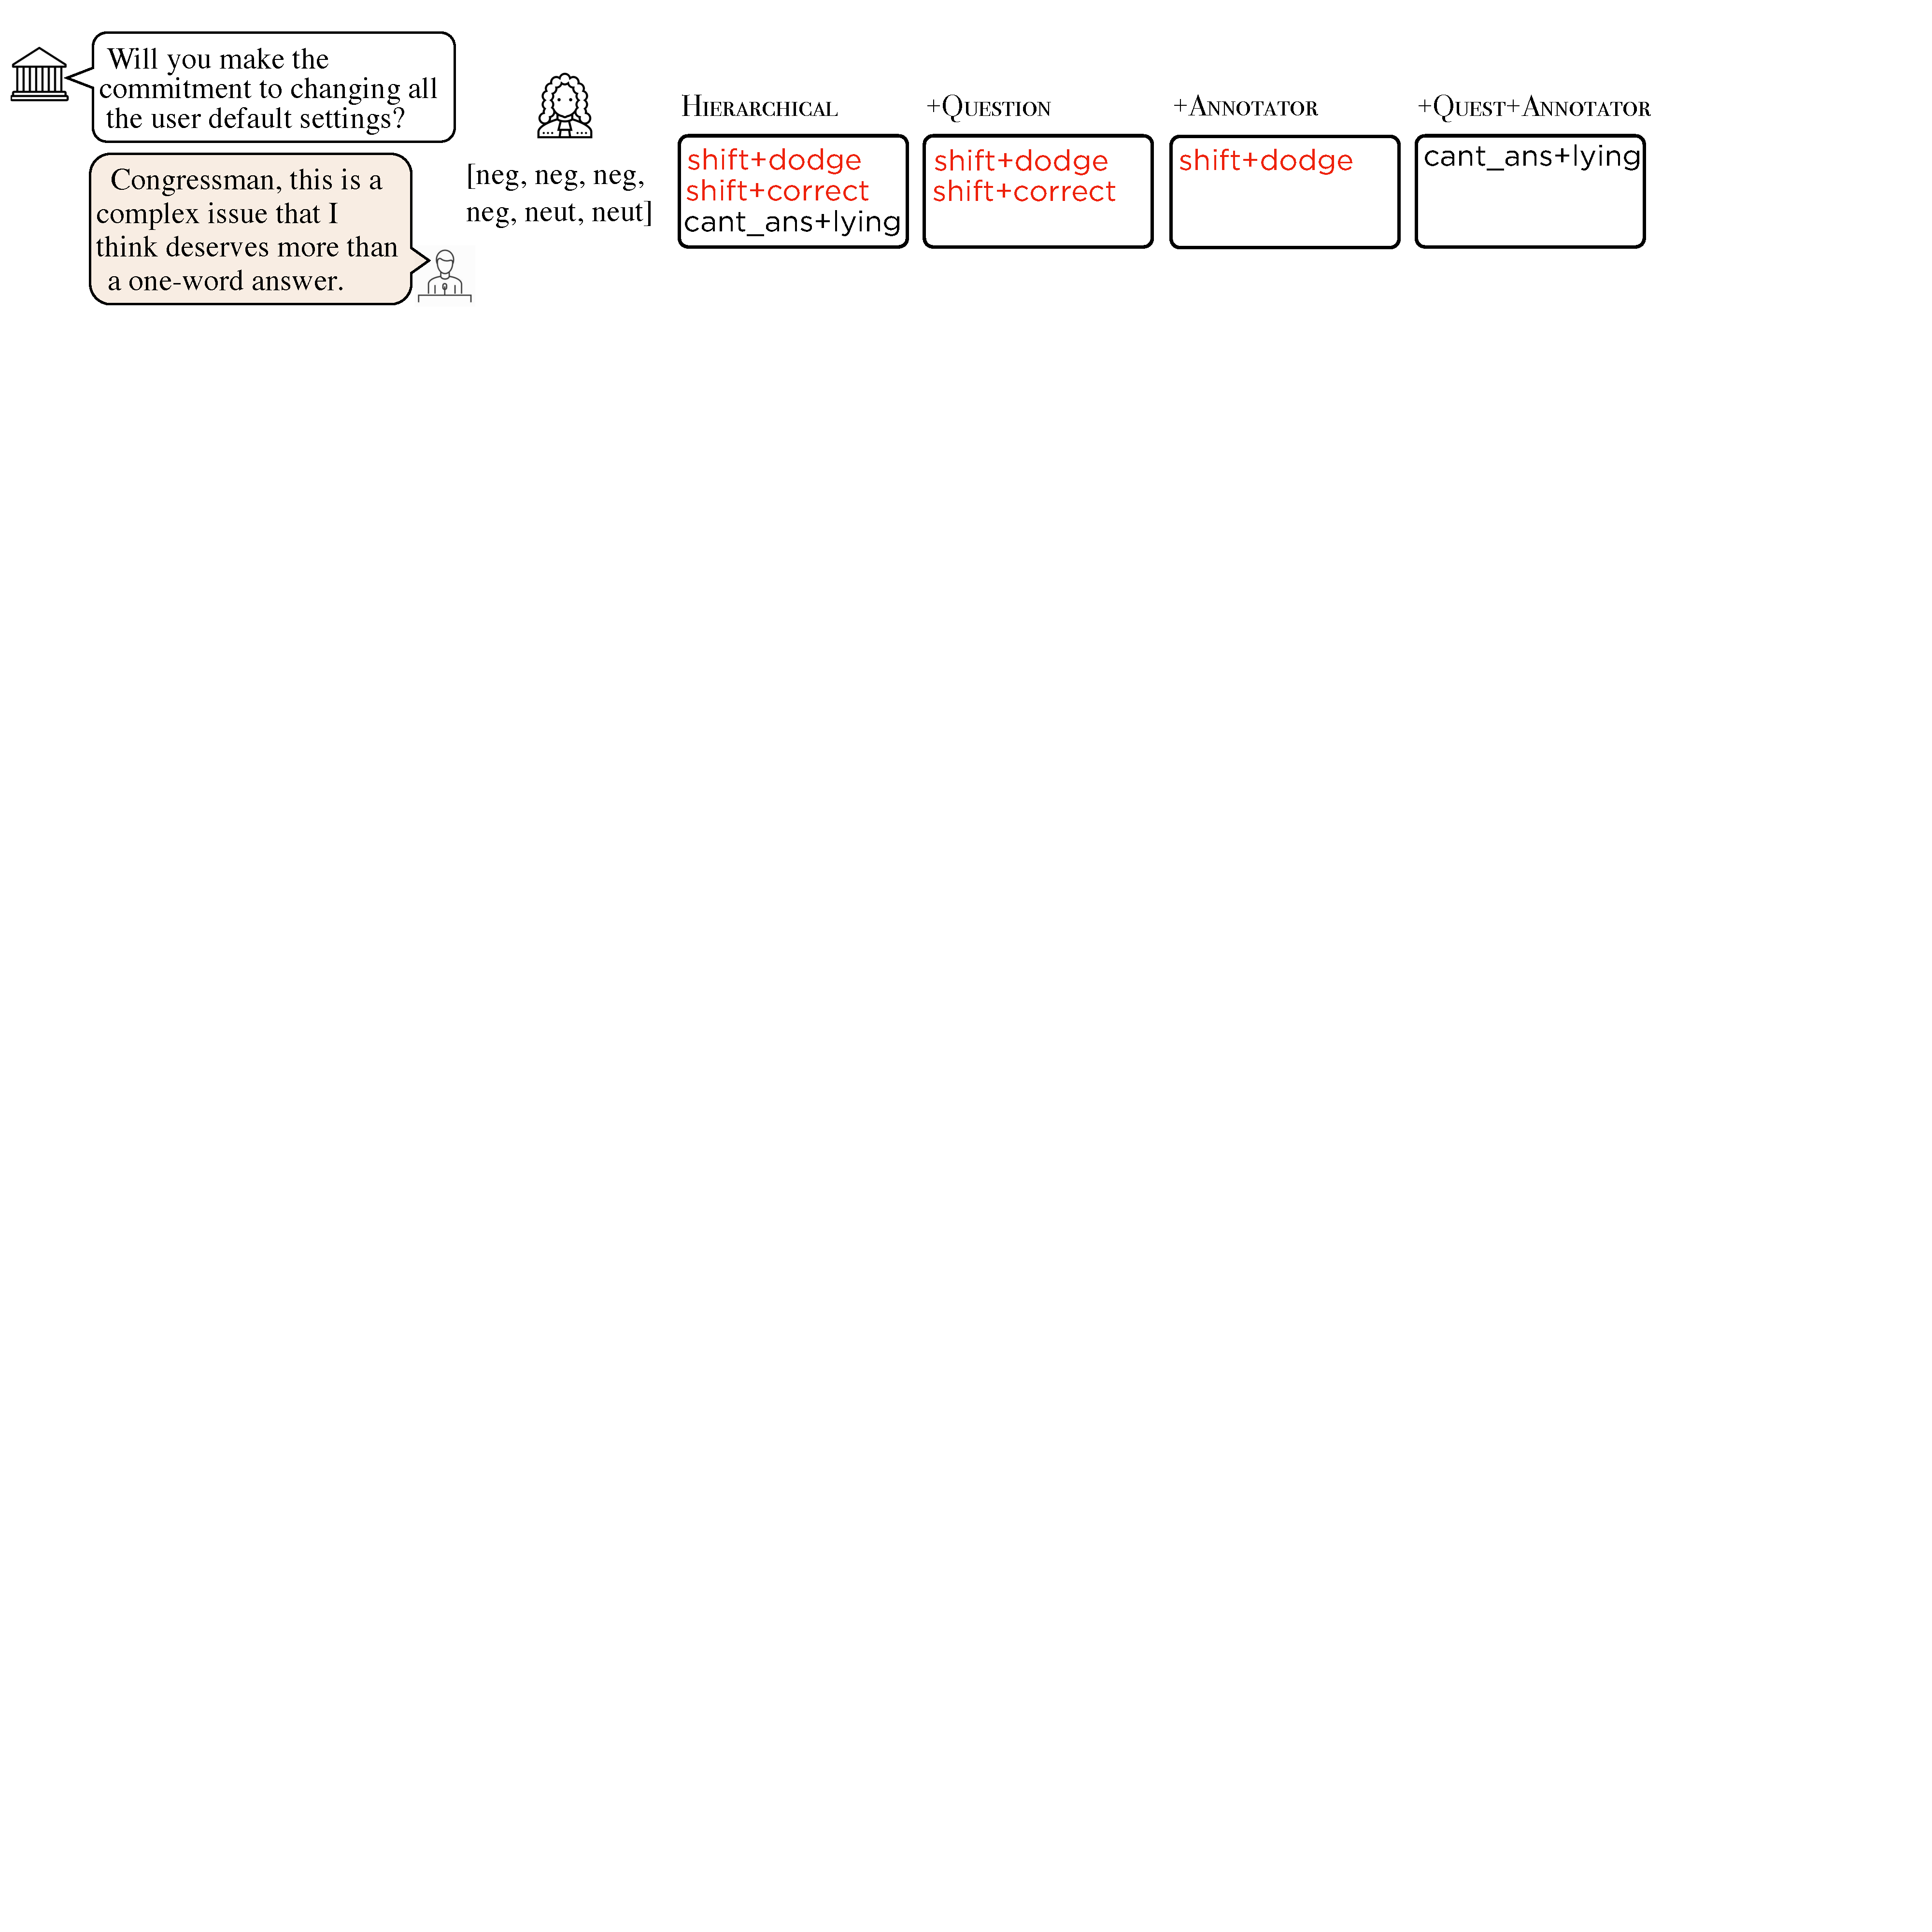
\includegraphics[scale=0.28]{plots/pred_models.pdf}
%     \vspace{-2.0em}
%     \caption{Predictions from the different models on a question-response pair with the shown annotator sentiments, where the final model correctly predicts all labels. Incorrect predictions are in red.}
%     \label{fig:pred_models}
% \end{figure}

\begin{table}[]
    \centering
    \scalebox{0.9}{
    \small
    \begin{tabular}{@{}>{\raggedright\arraybackslash}p{3.8cm}|>{\raggedright\arraybackslash}p{1.7cm}>{\raggedright\arraybackslash}p{1.7cm}>{\raggedright\arraybackslash}p{1.7cm}>{\raggedright\arraybackslash}p{2.1cm}@{}}
    \toprule
\multicolumn{1}{c}{Context} & \multicolumn{4}{c}{Model Predictions} \\
\midrule
\textbf{Question:} Will you make the commitment to changing all the user default settings?  & \textsc{Hierarch.} & \textsc{+Question} & \textsc{+Annotator} & \textsc{+Quest+Anno} \\
\textbf{Response:} Congressman, this is a complex issue that I think deserves more than a one-word answer. & \multirow{2}{*}{\parbox{2cm}{{\color{red}{shift+dodge shift+correct}} cant\_ans+lying}} & \multirow{2}{*}{\parbox{2cm}{{\color{red}{shift+dodge shift+correct}}}} & \multirow{2}{*}{{\color{red}{shift+dodge}}} & \multirow{2}{*}{cant\_ans+lying} \\
\textbf{Sentiments:} -1, -1, -1, -1, 0, 0 &  &  &  &\\
\bottomrule
    \end{tabular}}
    \caption{Model predictions as context is added, with incorrect labels in {\color{red}{red}}. In this example, adding the question creates a false negative, but adding the sentiments create a true negative. With both contexts, the model predicts the entire label set correctly.}
    \label{tab:pred_models}

\end{table}
\paragraph{Adding context} As shown in Table \ref{tab:subj_context_results}, adding the question in \textsc{+Question} provides a small (not significant) improvement by predicting the smallest class of \texttt{ans+overans} more frequently, resulting in a better false negative rate but at conversely at a higher false positive rate for this class. Additionally, the model underpredicts \texttt{cant\_ans+lying} as shown in the example of Table \ref{tab:pred_models} that misses this label. The lack of a significant benefit contradicts our expectations of the importance of the question and qualitative evidence that annotators do consider the question in their judgments (``it was a terrible question to begin with.'', as explained by one annotator), but it is consistent with the weak correlation results.

%We speculate the form of the question is a cue to whether or not an overanswer is warranted. Table \ref{tab:subj_context_examples} illustrates an example of a pointed question and a more open-ended question that are now predicted correctly by the last-question model.
Incorporating the annotator sentiments in \textsc{+Annotator} provides a bigger and significant benefit that helps the \texttt{ans+overans} class more effectively than the \textsc{+Question} model, where both the false positives and false negatives are improved. Additionally, the model improves on all the other smaller classes (\textsc{shift+correct}, \textsc{cant\_ans+lying}), as shown in Table \ref{tab:pred_models} where it corrects the false positive prediction made by the \textsc{Hierarchical} model.

We next attempt combining both contexts in \textsc{+Question+Annotator} to explore whether sentiment could aid the effectiveness of the question context. We find a small, but not significant improvement reflecting the strengths and weaknesses of each individual model. The combined model benefits from the better predictions on \texttt{ans+overans} from the \textsc{+Annotator} model, but also suffers from the poorer performance on \texttt{cant\_ans+lying} from the \textsc{+Question} model.

From these results, we conclude that our task is heavily contextual. On the one hand, linguistic features of the question are not strongly correlated with the response and our model is not able to make effective use of this information. On the other hand, we've shown annotator sentiment is not a simple reflection of intent but our model is able to extract a significant signal. Nevertheless, the disagreements appear to reflect other axes, and this work begins to scratch the surface of understanding the subjective conversation acts and intents of people.

\begin{figure}[t]
 \centering
 \vspace{-1.2em}
  \begin{subfigure}{.5\textwidth}
  \centering
  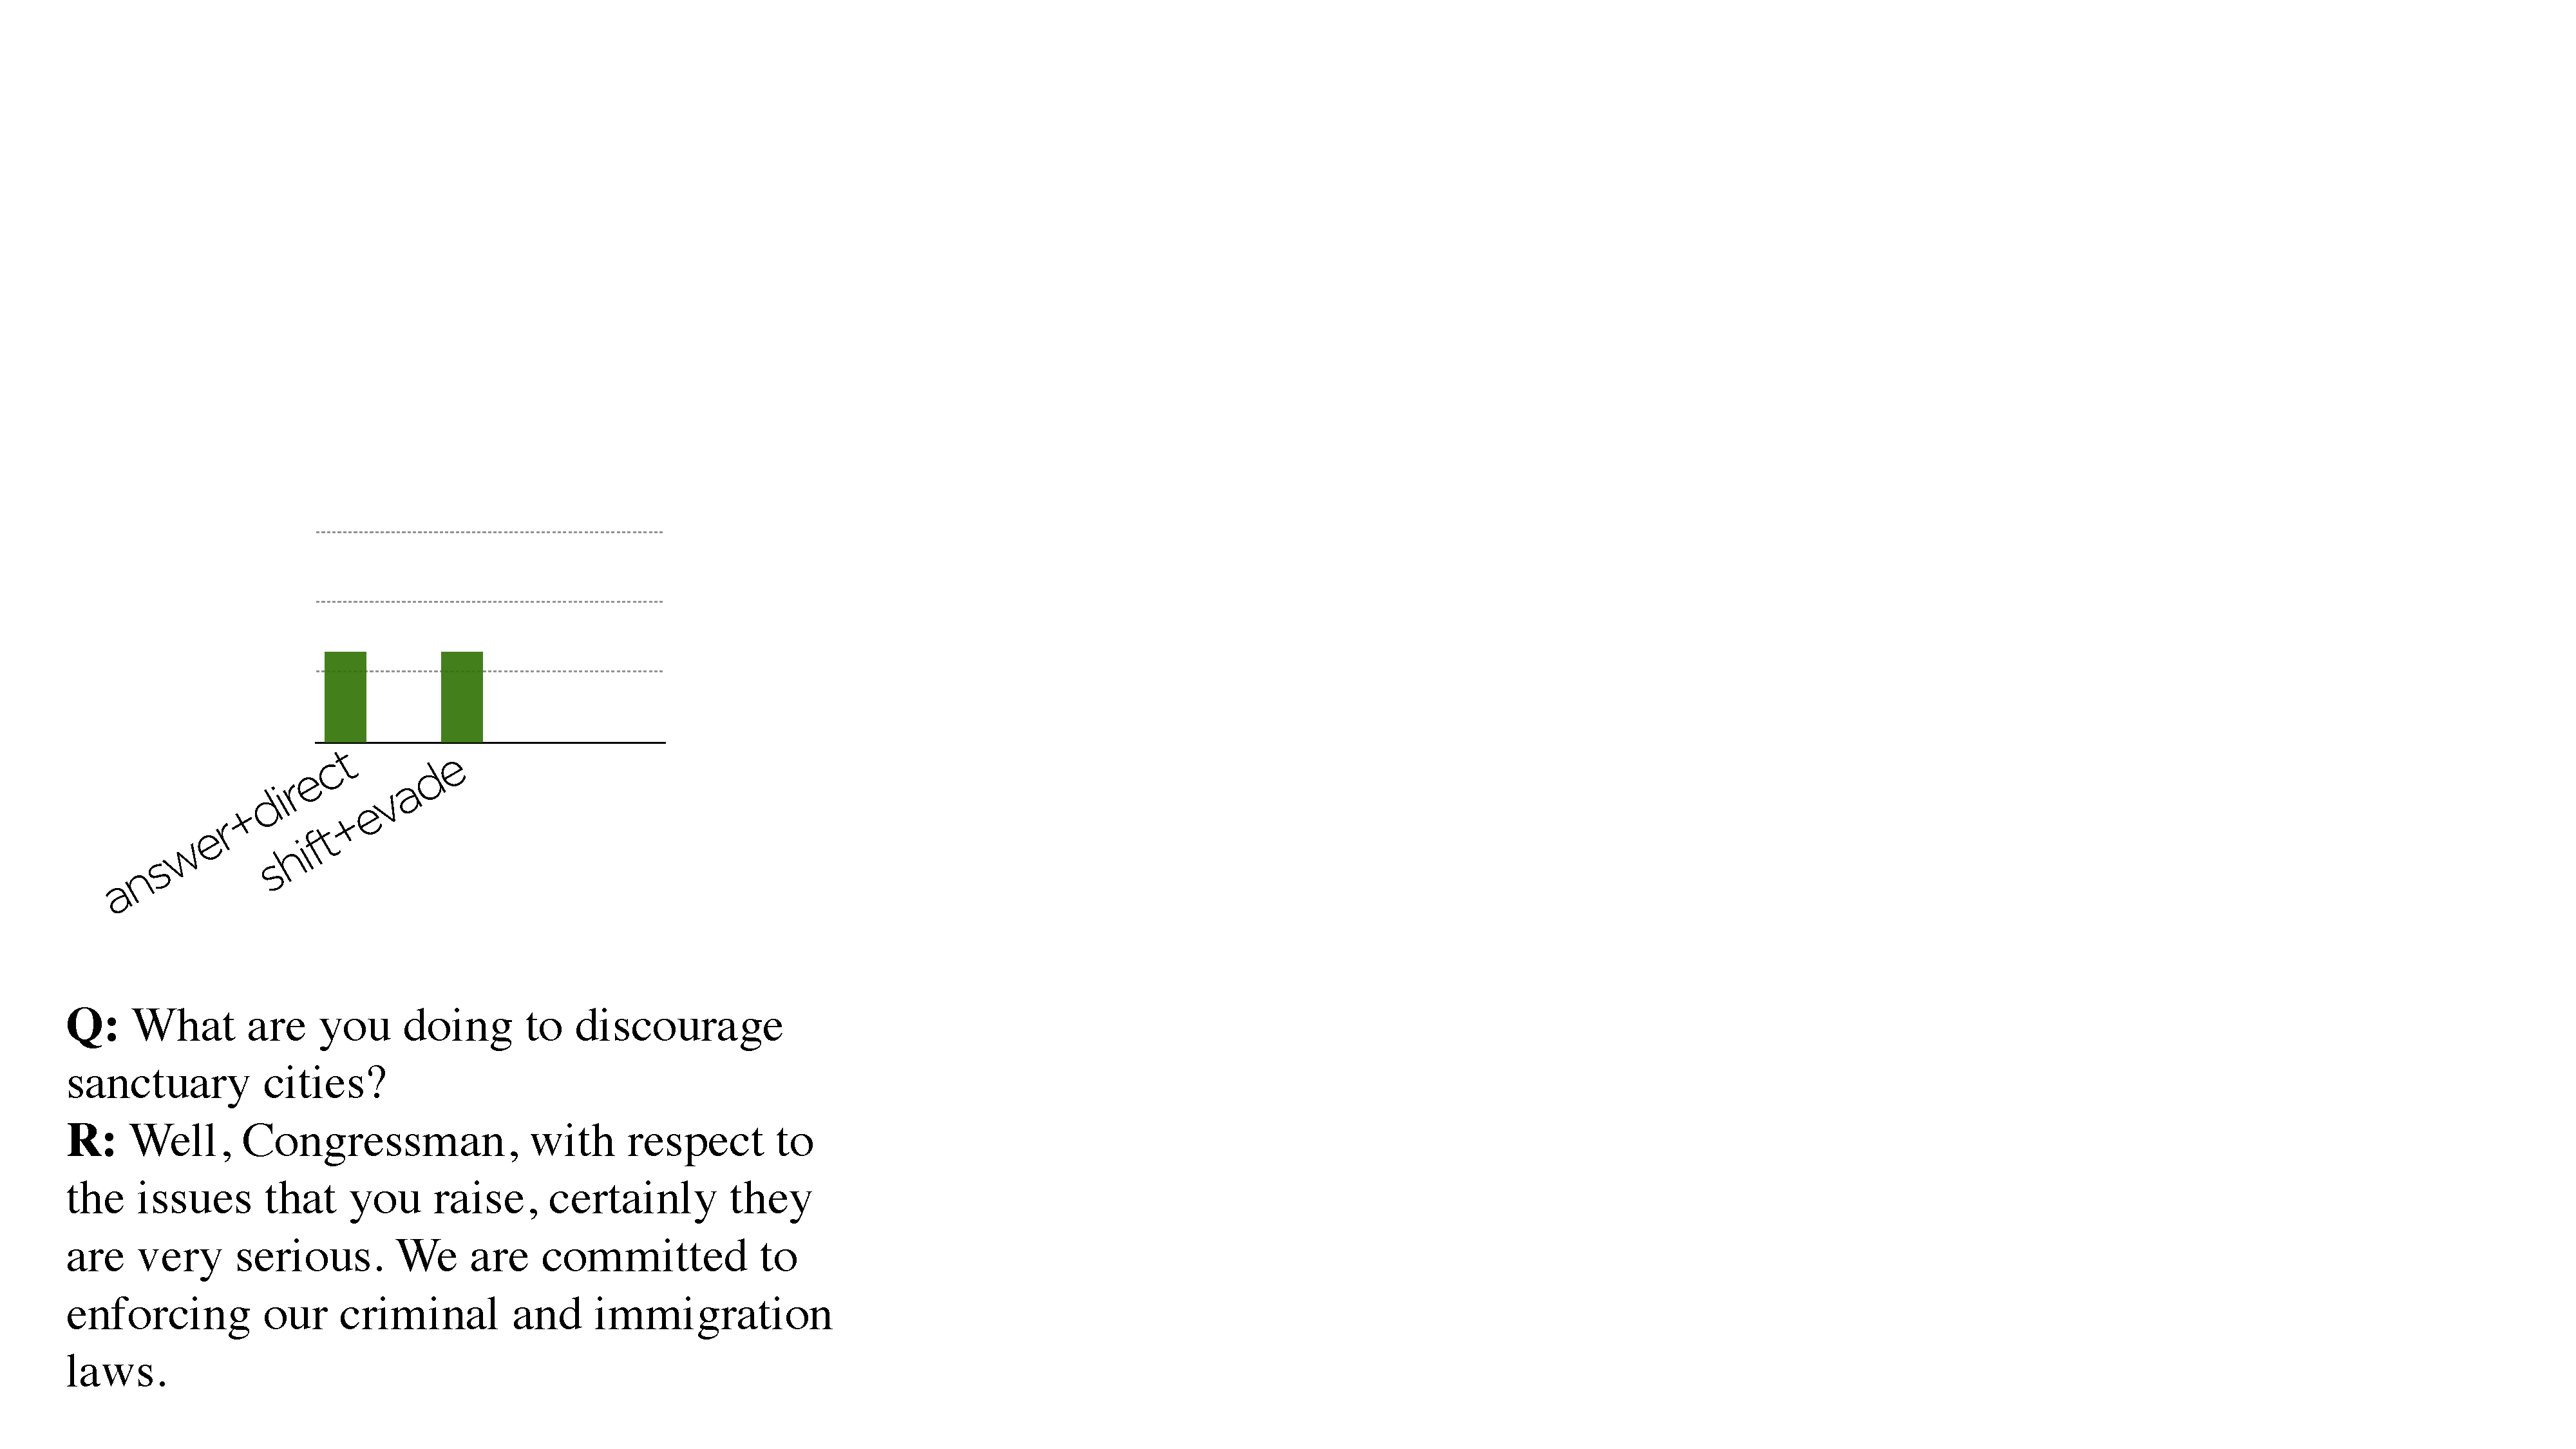
\includegraphics[scale=0.25]{plots/subj_level_disagree1.pdf}
  \vspace{-.3em}
  \caption{balanced disagreement (3 vs. 3)}
  \label{fig:subj_level_disagree_equal}
\end{subfigure}%
  \begin{subfigure}{.5\textwidth}
  \centering
  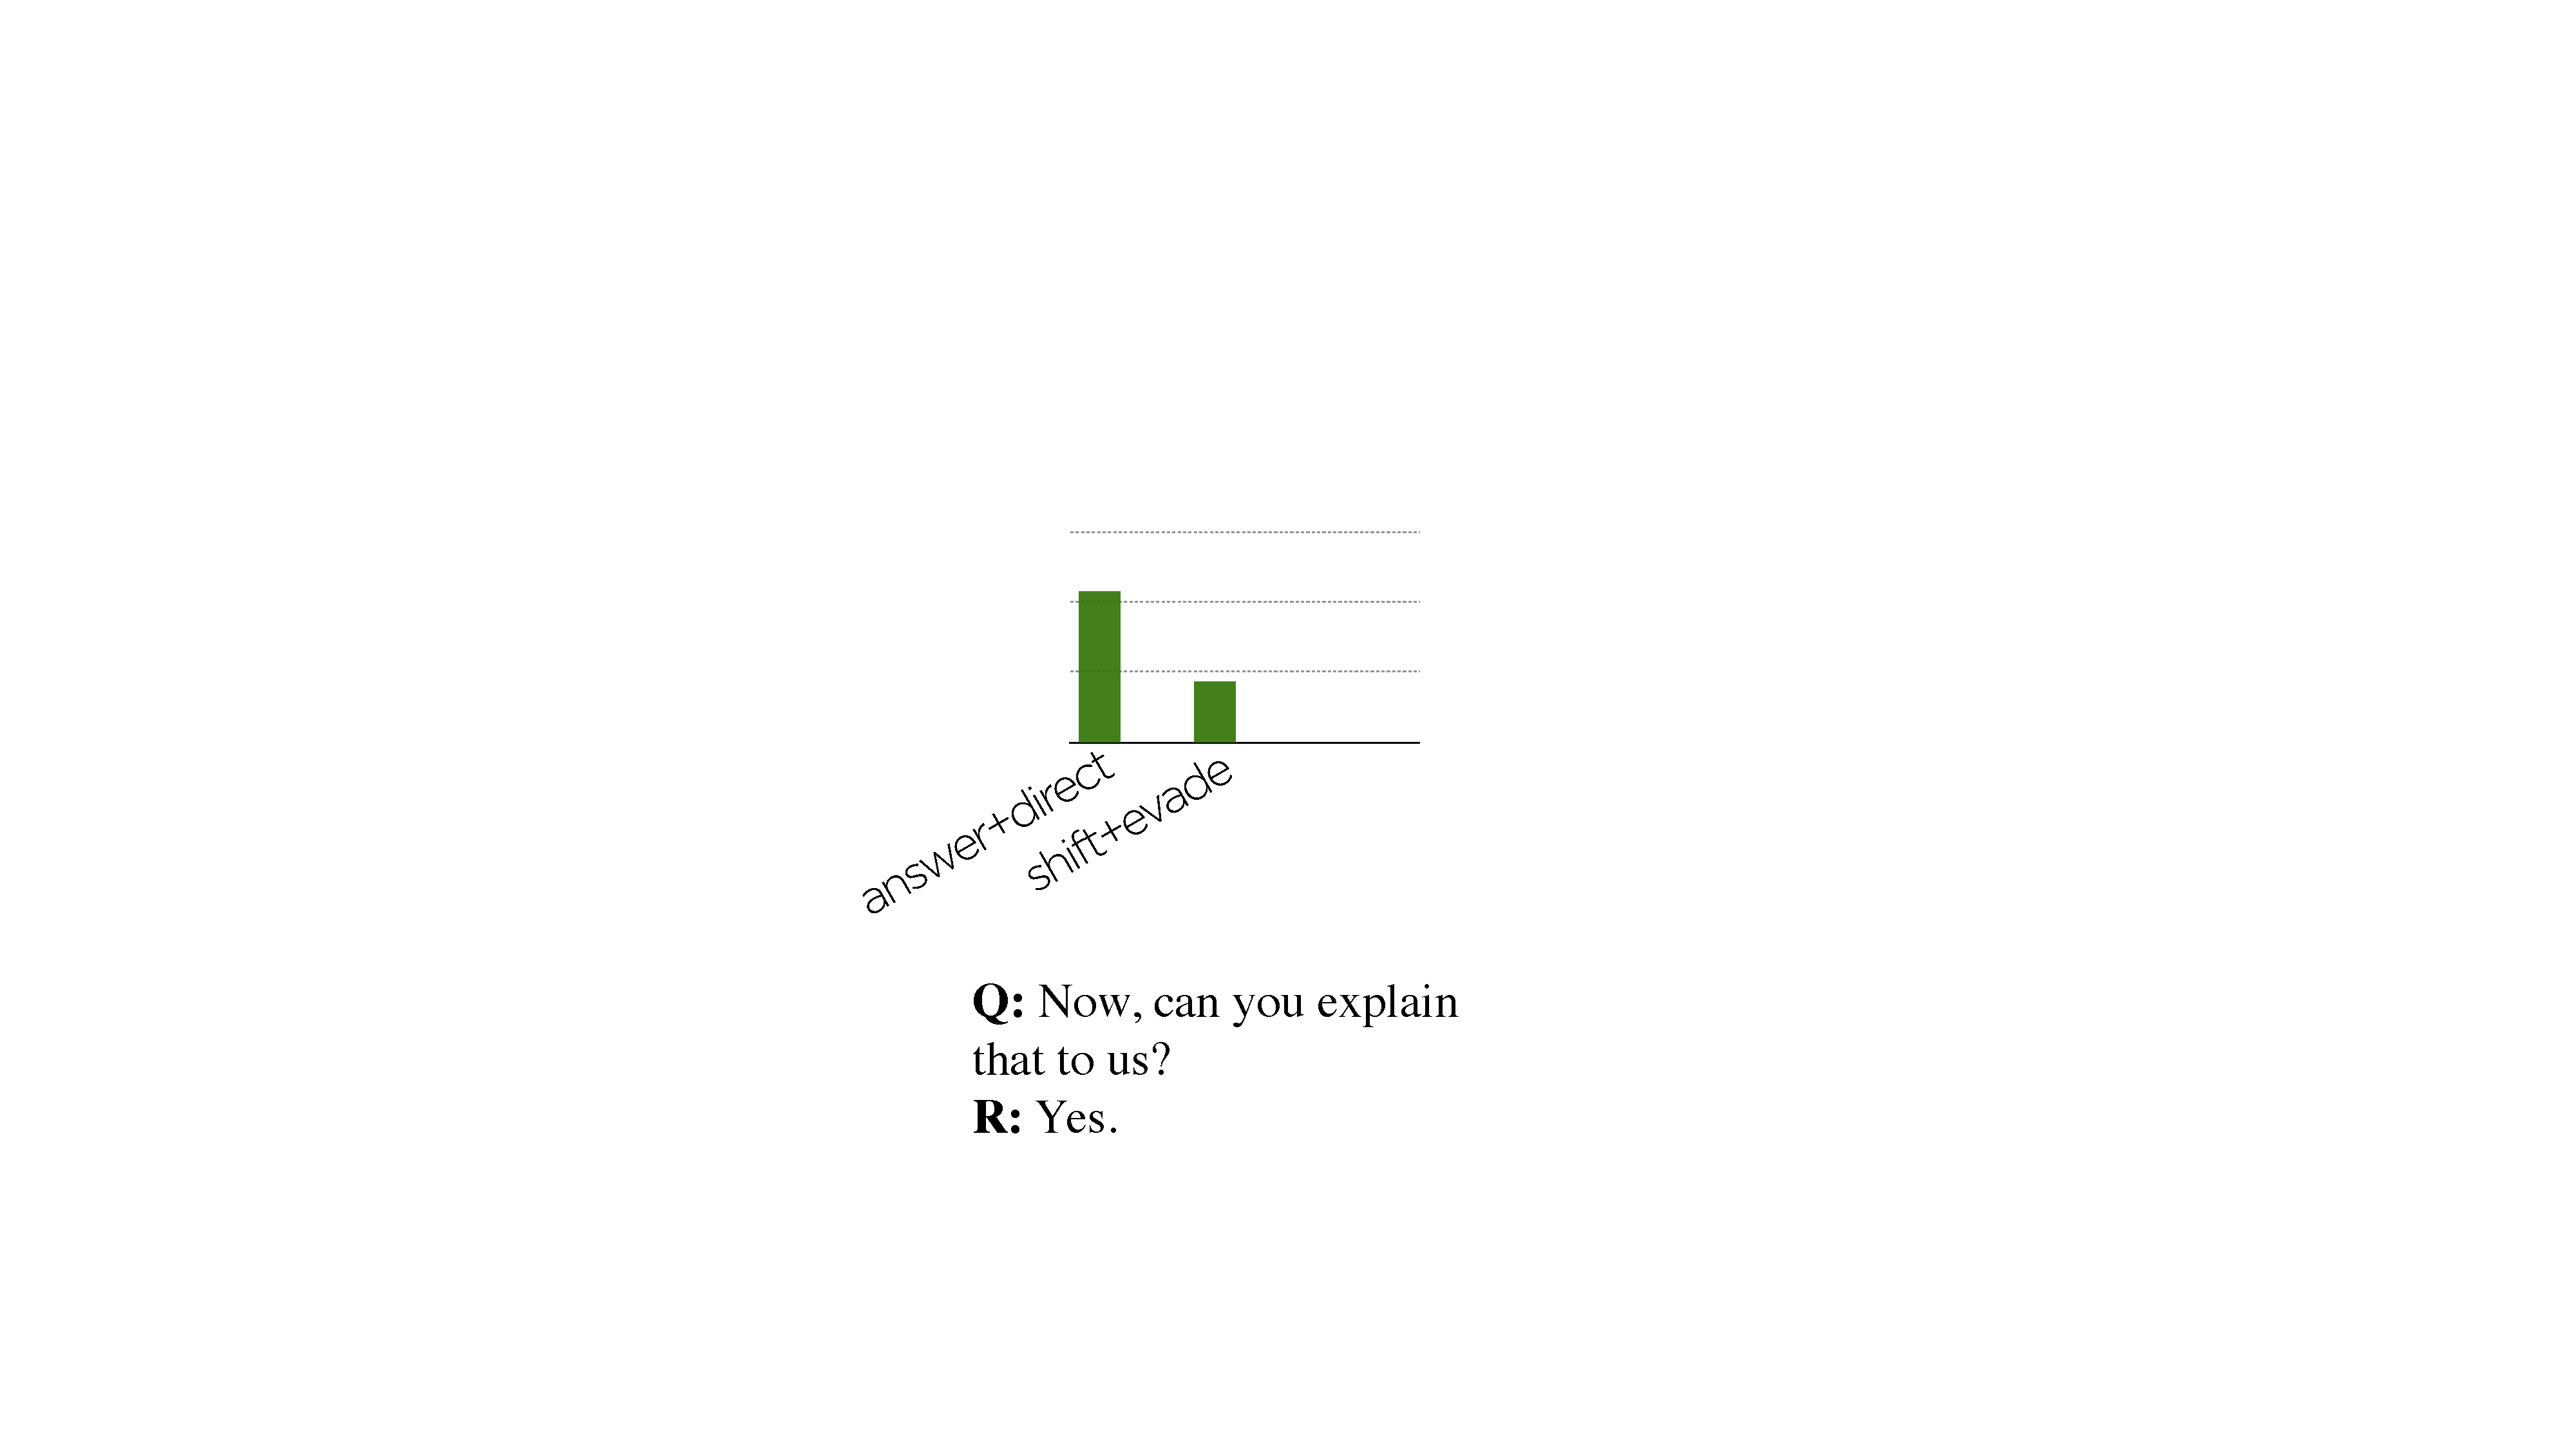
\includegraphics[scale=0.25]{plots/subj_level_disagree2.pdf}
  \vspace{-.3em}
  \caption{lop-sided disagreement (5 vs. 2)}
  \label{fig:subj_level_disagree_unequal}
\end{subfigure}
\vspace{-0.5em}
  \caption{Examples of question-response pairs with differing levels of agreement: judgments divided between two labels either equally (left) or or unequally (right.}
  \label{fig:subj_level_disagree}
  \vspace{-.3em}
\end{figure}

\section{Preliminary Experiment: Predicting the level of disagreement}
Our first task focused on predicting all possible interpretations, but is not able to distinguish between responses that elicit disagreements equally distributed among labels (Figure \ref{fig:subj_level_disagree_equal}), and responses that instead result in lop-sided judgments where only a minority interpret a certain label (Figure \ref{fig:subj_level_disagree_unequal}). These lop-sided cases could point to certain discourse that elicits more extreme or polarizing views. As a first step towards measuring the level of disagreement, we calculate the entropy over the labels for a given response.\footnote{An alternative approach is to use a bayesian model that pools together annotators with similar behaviors as in \newcite{Moreno:2015}, but modified to allow for multiple ground truths. We leave this exploration for future work.} The task of predicting the level of disagreement is framed as a regression problem.

\subsection{Models}
We present linear baselines and choose the strongest performing neural model from the previous task (\textsc{RoBERTa}). Models are evaluated with root mean squared error (RMSE) and Spearman's correlation $\rho$.

\paragraph{Training} Because this experiment is preliminary, we train and evaluate only on the held-out fold. Training details and hyperparameters are in Appendix \ref{sec:app_training}.

\paragraph{Baselines} We present two simple baselines: the \textsc{Majority} baseline predicts the most frequent entropy (0 for perfect agreement), and the \textsc{Mean} predicts the mean entropy over the held-out training dataset (0.34 after normalization). We also include the linear \textsc{Ridge} regression trained with bag-of-words representations.

\paragraph{RoBERTa} We modify the \textsc{RoBERTa} model for regression and perform a new hyperparameter grid search based on the best RMSE. 

\section{Results}
The pretrained \textsc{RoBERTa} model is able to outperform the baselines and linear model across both evaluation metrics, as shown in Table \ref{tab:subj_regression_results}. However, these results are still quite poor and a closer look at the predicted entropies in Figure \ref{fig:subj_entropies} shows they exhibit a very different distribution, clustering around the mean, and failing to predict even once the most frequent entropy value (0, which accounts for 49\% of the training data).

Although the model is able to fit to the training data, we suspect the MSE training objective has a strong prior to predict the mean when generalizing to unseen data. Because the entropy value fall into only one of nine categories, an alternative modeling approach we leave for future work is ordinal regression which retains the ordering between the different levels of disagreement. Furthermore the task of predicting the level of disagreement could be combined with the tasking of predicting the labels; for example, knowing all the possible labels could help predict the level of disagreement.

\begin{table}
    \centering
    \small
    \begin{tabular}{lll}
    \toprule
         Model &RMSE $\downarrow$ &Spearman's $\rho$ $\uparrow$ \\
         \midrule
         \textsc{Majority}&0.455 &-\\
         \textsc{Mean} &0.345 &-\\
         \textsc{Ridge} &0.290 &0.510 \\
         \midrule
         \textsc{RoBERTa} &\textbf{0.283} &\textbf{0.552}\\
         \bottomrule
    \end{tabular}
    \caption{Preliminary results for the regression task on the held-out development fold evaluated on RMSE (lower is better) and Spearman's correlation (higher is better).}
    \label{tab:subj_regression_results}
\end{table}

\begin{figure}[b]
 \centering
 \vspace{-1.2em}
  \begin{subfigure}{.5\textwidth}
  \centering
  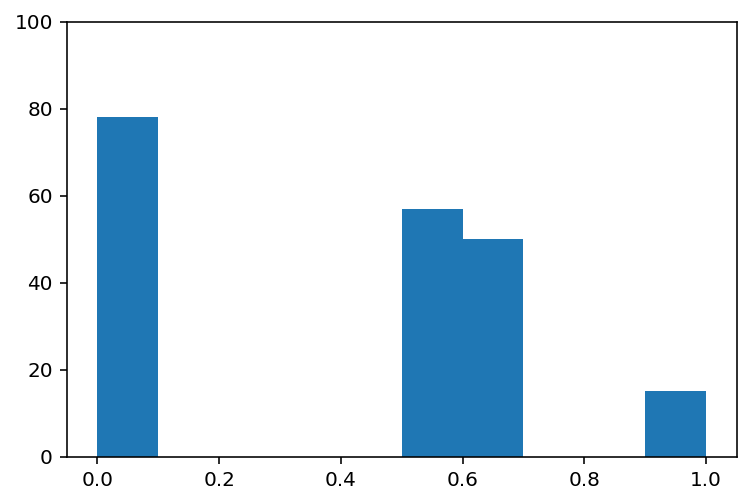
\includegraphics[scale=0.3]{plots/subj_entropy_golds.png}
  \vspace{-.3em}
  \caption{gold}
\end{subfigure}%
  \begin{subfigure}{.5\textwidth}
  \centering
  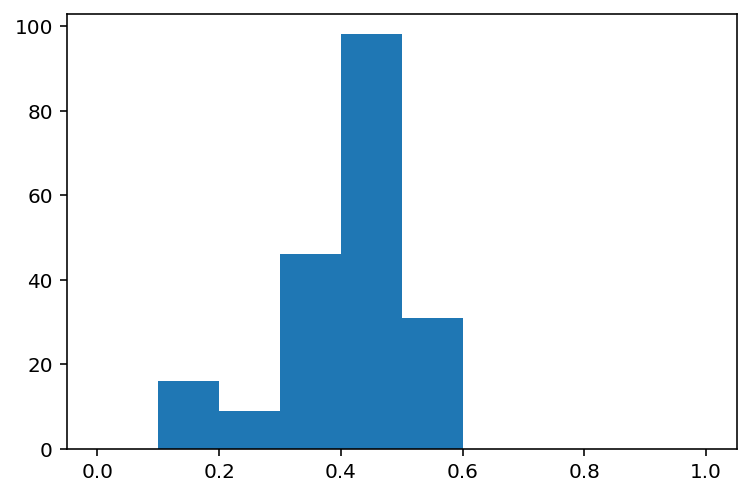
\includegraphics[scale=0.3]{plots/subj_entropy_preds.png}
  \vspace{-.3em}
  \caption{predicted}
\end{subfigure}
\vspace{-0.5em}
  \caption{Histograms for gold (left) vs. predicted entropies (right) that show predictions cluster around the mean and are never able to predict the most frequent value (0).}
  \label{fig:subj_entropies}
  \vspace{-.3em}
\end{figure}

\section{Chapter Summary}

In this chapter, we tackle the \emph{subjectivity} of discourse; that is, how ambiguities are resolved. We present a novel English dataset containing \emph{multiple} ground truths in the form of subjective judgments on the conversation acts and intents of a response in a question-response setting. We show the dataset contains genuine disagreements which turn out to be complex and not easily attributable to a single feature, such as annotator sentiment. The annotator rationales provide a window into understanding these complexities, and offer a rich source of linguistic devices. We propose a task to predict all possible interpretations of a response, whose results are consistent with our data analysis: incorporating both the context of the question and the annotator bias helps the model significantly improve. We also present preliminary results on predicting the level of disagreement, where we find much room for improvement. We publicly release the dataset in hopes to spur further research.

